\باب{کثیر المتغیر تفاعل اور جزوی تفرقات}
\موٹا{جائزہ}\\
سائنس میں دو یا دو سے زائد غیر تابع  متغیرات کے تفاعل    ایک متغیر کے تفاعل سے زیادہ کثرت سے پائے جاتے ہیں اور ان کی علم   احصاء  زیادہ  عمدہ   ہوتی  ہے۔زیادہ متغیرات ایک دوسرے پر زیادہ طریقوں سے اثر انداز ہو سکتے ہیں جس کی بنا ان کے تفرقات    مختلف اور زیادہ دلچسپ  صورتیں اختیار  کر سکتے ہیں۔ ان کے تکملات  زیادہ اقسام کے عملی  مسائل میں کام آتے ہیں۔ احتمال،  سیالی حرکیات، اور برقیات، وغیرہ،    پر غور کے دوران  ایک سے زائد متغیرات  کے تفاعل قدرتی طور پر رونما ہوتے ہیں۔ان تفاعل کی  ریاضیات، سائنس کی عظیم  کامیابیوں میں  سے ایک ہے۔


\حصہ{کثیر متغیرات کے تفاعل}
کئی تفاعل ایک سے زائد متغیرات کے تابع  ہوتے ہیں۔دائری نلکی کا حجم،  اس    کے رداس اور قد سے،   تفاعل  \عددی{H=\pi r^2h}   دیتا ہے۔ مستوی \عددی{xy} میں نقطہ \عددی{N(x,y)} کے دو محدد سے،   قطع مکافی   \عددی{z=x^2+y^2}  کا قد  تفاعل \عددی{f(x,y)=x^2+y^2} دیتا ہے۔اس حصہ میں ہم ایک سے زیادہ متغیرات کے تابع تفاعل متعارف کرتے ہیں  اور ان کو ترسیم کرنے کے طریقوں پر غور کرتے ہیں۔

\جزوحصہء{تفاعل اور متغیرات} 
کثیر غیر تابع حقیقی متغیرات  کے حقیقی قیمت تفاعل کی تعریف  بالکل واحد متغیر کے تفاعل کی طرح کی جاتی ہے۔ان کے وقفے  حقیقی   (تین، چار، وغیرہ)    اعداد کے  مرتب جوڑی  کے سلسلے ہوں گے اور ان  کی  سعت  ، اس طرح  کے حقیقی اعداد کے سلسلے ہوں گے جن کے ساتھ ہم کام کرتے آ رہے ہیں۔

\ابتدا{تعریفات}
فرض کریں \عددی{n} عدد حقیقی اعداد \عددی{x_1,x_2,\cdots,x_n} کا سلسلہ \عددی{D} ہے۔  تب \عددی{D} پر \اصطلاح{حقیقی قیمت تفاعل}\فرہنگ{تفاعل!حقیقی قیمت}\حاشیہب{real valued function}\فرہنگ{function!real valued} \عددی{f} سے مراد وہ قاعدہ ہے جو \عددی{D} کے ہر رکن کو حقیقی عدد
\begin{align*}
w=f(x_1,x_2,\cdots,x_n)
\end{align*}
مختص کرتا ہو۔سلسلہ \عددی{D} اس تفاعل کا \اصطلاح{دائرہ کار}\فرہنگ{دائرہ کار}\حاشیہب{domain}\فرہنگ{domain} ہو گا۔  تفاعل  \عددی{f} کی  \عددی{w} قیمتوں کا سلسلہ  \عددی{f} کی \اصطلاح{سعت}\فرہنگ{سعت}\حاشیہب{range}\فرہنگ{range} ہو گی۔ علامت \عددی{w} تفاعل \عددی{f} کا \اصطلاح{تابع متغیر}\فرہنگ{متغیر!تابع}\حاشیہب{dependent variable}\فرہنگ{variable!dependent} ہو گا اور \عددی{f} کو  \عددی{n}  \اصطلاح{غیر تابع متغیرات}\فرہنگ{متغیر!غیر تابع}\حاشیہب{independent variable}\فرہنگ{variable!independent} \عددی{x_1} تا \عددی{x_n}   کا تفاعل کہتے ہیں۔ ہم  ان \عددی{x} کو تفاعل کے \اصطلاح{داخلی متغیرات}\فرہنگ{متغیر!داخلی}\حاشیہب{input variable}\فرہنگ{variable!input} اور \عددی{w} کو تفاعل کا \اصطلاح{خارجی متغیر}\فرہنگ{متغیر!خارجی}\حاشیہب{output variable}\فرہنگ{variable!output}  بھی کہتے ہیں۔
\انتہا{تعریفات}
%==================

اگر \عددی{f} دو غیر تابع متغیرات کا تفاعل ہو تب عموماً ہم  ان غیر تابع متغیرات کو \عددی{x} اور \عددی{y} کہتے ہیں اور \عددی{f} کے دائرہ کار  کو مستوی \عددی{xy} میں ایک خطہ تصور کرتے ہیں۔ اگر \عددی{f} تین غیر تابع متغیرات کا تفاعل ہو تب ہم  ان متغیرات کو \عددی{x}، \عددی{y} اور \عددی{z} کہتے ہیں اور تفاعل کے  دائرہ کار کو فضا میں ایک خطہ تصور کرتے ہیں۔

عملی استعمال میں ہم  وہ حروف استعمال کرتے ہیں جو ہمیں ان چیزوں  کی یاد  دلا سکیں جن کے لئے یہ متغیرات استعمال  کیے گئے ہوں۔ یہ  کہنے  کی خاطر کہ دائری نلکی کا حجم اس کے رداس \عددی{r}  اور قد \عددی{h}   کا تفاعل ہو گا، ہم \عددی{H=f(r,h)} لکھ سکتے ہیں۔بالخصوص  ہم \عددی{f(r,h)} کی جگہ وہ کلیہ استعمال کر سکتے ہیں جو \عددی{r} اور \عددی{h} کی قیمتوں سے \عددی{H} کی  قیمت دیتا ہو، یعنی ہم  \عددی{H=\pi r^2h} لکھ سکتے ہیں۔دونوں صورتوں میں \عددی{r} اور \عددی{h} غیر تابع متغیرات ہوں گے اور \عددی{H} تابع متغیر ہو گا۔

ہمیشہ کی طرح،ہم  تفاعل کی تعریفی کلیہ میں غیر تابع متغیرات کی قیمتیں پر کر  کے مطابقتی تابع متغیر کی قیمت حاصل کرتے ہیں۔

\ابتدا{مثال}
نقطہ \عددی{(3,0,4)} پر تفاعل \عددی{f(x,y,z)=\sqrt{x^2+y^2+z^2}} کی قیمت درج ذیل ہو گی۔
\begin{align*}
f(3,0,4)=\sqrt{(3)^2+(0)^2+(4)^2}=\sqrt{25}=5
\end{align*}
\انتہا{مثال}
%===============
\جزوحصہء{وقفے}
ایک سے زیادہ متغیرات کے تفاعل  کی تعریف  میں، ہمیشہ کی طرح، ہم  ان مداخل کو  شامل نہیں  کرتے ہیں  جو مخلوط اعداد دیتے ہوں یا جن کی وجہ سے   تقسیم صفر  کا عمل  پیدا ہوتا ہو۔یوں \عددی{f(x,y)=\sqrt{y-x^2}} میں \عددی{y} کی قیمت \عددی{x^2} کی قیمت سے کم نہیں ہو سکتی ہے اور \عددی{f(x,y)=\tfrac{1}{xy}} میں \عددی{xy} کی قیمت صفر نہیں ہو سکتی ہے۔ان شرائط کو مطمئن کرتے ہوئے، تفاعل کے  دائرہ کار سے مراد  وہ بڑے سے بڑا سلسلہ ہو گا جس پر تفاعل کا  تعریفی قاعدہ حقیقی اعداد  پیدا کرتا ہو۔ 

\ابتدا{مثال}\ترچھا{دو متغیرات کے تفاعل}\\
\begin{center}
\renewcommand{\arraystretch}{1.2} 
\begin{tabular}{LLL}
\multicolumn{1}{C}{\text{\RL{تفاعل}}}&\text{\RL{دائرہ کار}}&\multicolumn{1}{C}{\text{\RL{سعت}}}\\
\midrule
w=\sqrt{y-x^2}&y\ge x^2&[0,\infty)\\
w=\tfrac{1}{xy}&xy\ne 0&(-\infty,0)\cup(0,\infty)\\
w=\sin xy&\text{\RL{پورا مستوی}}&[-1,1]
\end{tabular}
\end{center}
\انتہا{مثال}
%===============
\ابتدا{مثال}\ترچھا{تین متغیرات کے  تفاعل}\\
\begin{center}
\renewcommand{\arraystretch}{1.2} 
\begin{tabular}{LLL}
\multicolumn{1}{C}{\text{\RL{تفاعل}}}&\multicolumn{1}{C}{\text{\RL{دائرہ کار}}}&\multicolumn{1}{C}{\text{\RL{سعت}}}\\
\midrule
w=\sqrt{x^2+y^2+z^2}&\text{\RL{پوری فضا}}&[0,\infty)\\
w=\dfrac{1}{x^2+y^2+z^2}&(x,y,z)\ne (0,0,0)&(0,\infty)\\
w=xy\ln z&\text{\RL{نصف فضا z>0}}&(-\infty,\infty)
\end{tabular}
\end{center}
\انتہا{مثال}
%===========
بالکل حقیقی لکیر کے وقفوں  پر معین تفاعل کے دائرہ کار کی طرح، مستوی  کے حصوں پر معین تفاعل کے دائرہ کار کے اندرونی نقطے اور  سرحدی نقطے  ہو سکتے ہیں۔
\begin{figure}
\centering
\begin{subfigure}{0.45\textwidth}
\centering
\begin{tikzpicture}[scale=0.75]
\draw[smooth cycle,fill=llgray]plot coordinates {(0,0)(1,-2)(2,-1.5)(3,-2)(5,-1)(4.5,0)(5,1)(2,2)(1,1.5)};
\draw[dashed,fill=lgray](3,-0.5)node[circ]{}node[pin={[pin edge=solid]135:{$(x_0,y_0)$}}]{} circle (0.5);
\draw(1,-1)node[]{$R$};
\end{tikzpicture}
\caption{اندرونی نقطہ}
\end{subfigure}\hfill
\begin{subfigure}{0.45\textwidth}
\centering
\begin{tikzpicture}[scale=0.75]
\draw[name path=kout,smooth cycle,fill=llgray]plot coordinates {(0,0)(1,-2)(2,-1.5)(3,-2)(5,-1)(4.5,0)(5,1)(2,2)(1,1.5)};
\draw(1,-1)node[]{$R$};
\begin{scope}
\path[clip,smooth cycle]plot coordinates {(0,0)(1,-2)(2,-1.5)(3,-2)(5,-1)(4.5,0)(5,1)(2,2)(1,1.5)};
\fill[lgray](3,-2) circle (0.5);
\end{scope}
\draw[dashed,name path=kin](3,-2)node[circ]{}node[pin={[pin edge=solid,above]70:{$(x_0,y_0)$}}]{} circle (0.5);
\end{tikzpicture}
\caption{سرحدی  نقطہ}
\end{subfigure}
\caption{مستوی خطہ \عددی{R}  کا اندرونی نقطہ اور سرحدی نقطہ۔اندرونی نقطہ لازماً \عددی{R} کا حصہ ہو گا جبکہ ضروری نہیں کہ سرحدی نقطہ \عددی{} کا حصہ ہو۔}
\label{شکل_کثیرالمتغیر_اندرونی_سرحدی_نقاط}
\end{figure}

\ابتدا{تعریفات}
مستوی \عددی{xy} میں خطہ (سلسلہ) \عددی{R}  میں نقطہ \عددی{(x_0,y_0)}  تب \عددی{R} کا \اصطلاح{اندرونی نقطہ}\فرہنگ{نقطہ!اندرونی}\حاشیہب{interior point}\فرہنگ{point!interior} ہو گا جب  یہ اس قرص کا مرکز  ہو جو مکمل طور پر \عددی{R} میں پایا جاتا ہو (شکل \حوالہ{شکل_کثیرالمتغیر_اندرونی_سرحدی_نقاط})۔  نقطہ \عددی{(x_0,y_0)} تب \عددی{R} کا  \اصطلاح{سرحدی نقطہ}\فرہنگ{نقطہ!سرحدی}\حاشیہب{boundary point}\فرہنگ{point!boundary} ہو گا جب ہر اس  قرص  میں، جس کا مرکز \عددی{(x_0,y_0)} ہو ،  \عددی{R} کے بیرونی  اور \عددی{R} کے اندرونی نقطے پائے جاتے ہوں۔(ضروری نہیں کہ سرحدی نقطہ ازخود \عددی{R} میں شامل  ہو۔ )

ایک خطہ کے اندرونی نقطے، بطور ایک سلسلہ، اس خطہ  کی\اصطلاح{ اندرون}\فرہنگ{اندرون}\حاشیہب{interior}\فرہنگ{interior} ہوں گے۔ اس خطہ کے سرحدی نقطے اس کی \اصطلاح{سرحد}\فرہنگ{سرحد}\حاشیہب{boundary}\فرہنگ{boundary}  ہیں۔ایسا خطہ  جو مکمل طور پر اندرونی نقطوں پر مشتمل ہو \اصطلاح{کھلا}\فرہنگ{کھلا}\حاشیہب{open}\فرہنگ{open} خطہ کہلاتا ہے۔ ایسا خطہ جس میں  اس کے تمام سرحدی نقطے شامل ہوں \اصطلاح{بند}\فرہنگ{بند}\حاشیہب{closed}\فرہنگ{closed} خطہ کہلاتا ہے۔ 
\انتہا{تعریفات}
%===================
\begin{figure}
\centering
\begin{subfigure}{0.30\textwidth}
\centering
\begin{tikzpicture}
\draw(0,0)node[below left]{$O$};
\fill[llgray](0,0) circle (1);
\draw[dashed,fill=lgray](0.4,0.4)node[circ]{} circle (0.25);
\draw[-latex](-1.5,0)--(1.5,0)node[right]{$x$};
\draw[-latex](0,-1.25)--(0,1.5)node[left]{$y$};
\end{tikzpicture}
\caption{
\عددی{\{(x,y)|x^2+y^2<1\}}\\
کھلا قرص۔ ہر نقطہ اندرونی نقطہ ہے۔
}
\end{subfigure}\hfill
\begin{subfigure}{0.30\textwidth}
\centering
\begin{tikzpicture}
\draw(0,0)node[below left]{$O$};
\begin{scope}
\draw[clip](0,0) circle (1);
\fill[lgray](45:1) circle (0.25);
\end{scope}
\draw[dashed](45:1)node[circ]{} circle (0.25);
\draw[-latex](-1.5,0)--(1.5,0)node[right]{$x$};
\draw[-latex](0,-1.25)--(0,1.5)node[left]{$y$};
\end{tikzpicture}
\caption{
\عددی{\{(x,y)|x^2+y^2=1\}}\\
اکائی قرص کی  سرحد۔ (اکائی دائرہ۔)
}
\end{subfigure}\hfill
\begin{subfigure}{0.30\textwidth}
\centering
\begin{tikzpicture}
\draw(0,0)node[below left]{$O$};
\draw[fill=llgray](0,0) circle (1);
\draw[-latex](-1.5,0)--(1.5,0)node[right]{$x$};
\draw[-latex](0,-1.25)--(0,1.5)node[left]{$y$};
\end{tikzpicture}
\caption{
\عددی{\{(x,y)|x^2+y^2\le 1\}}\\
بند اکائی قرص۔تمام سرحدی نقطے اس میں شامل ہیں۔
}
\end{subfigure}
\caption{مستوی میں اکائی قرص کے اندرونی نقطے اور سرحدی نقطے۔}
\label{شکل_کثیرالمتغیر_اکائی_قرص_اندرونی_سرحدی}
\end{figure}

حقیقی اعداد کے وقفوں کی طرح، مستوی میں بعض خطے نا کھلا اور نا ہی بند ہوتے ہیں۔ شکل \حوالہ{شکل_کثیرالمتغیر_اکائی_قرص_اندرونی_سرحدی} کے کھلا قرص   میں چند،   نا کہ  تمام،    سرحدی نقطے شامل کرنے سے ایسا خطہ حاصل ہو گا جو نا کھلا ہو گا اور نا ہی بند ہو گا۔اس میں شامل سرحدی نقطے اس کو کھلا وقفہ بننے  سے روکتے  ہیں جبکہ اس میں نا  شامل سرحدی نقطے اس کو  بند  خطہ بننے سے روکتے ہیں۔

\ابتدا{تعریف}
مستوی میں  مقررہ رداس کے قرص  میں پائے جانے والا خطہ  \اصطلاح{محدود}\فرہنگ{محدود}\حاشیہب{bounded}\فرہنگ{bounded} ہو گا۔  ایسا خطہ جو محدود نا ہو \اصطلاح{غیر محدود}\فرہنگ{غیر محدود}\حاشیہب{unbounded}\فرہنگ{unbounded}  ہو گا۔
\انتہا{تعریف}
%================
\begin{figure}
\centering
\begin{tikzpicture}[font=\small,declare function={f(\x)=(\x)^2;}]
 \pgfmathsetseed{42}
\begin{axis}[clip=false,axis on top,small,axis lines=middle,xtick={-1,1},ytick={1},enlargelimits=true,xlabel={$x$},ylabel={$y$},xlabel style={at={(current axis.right of origin)},anchor=north},ylabel style={at={(current axis.above origin)},anchor=south}]
\addplot[thick,name path=kc,domain=-2:2]{f(x)}node[pos=0.85,pin={[align=right,below]-45:{\RL{قطع مکافی}\\ $y-x^2=0$\\   \RL{سرحد ہے}}}]{};
    \draw[name path=kl,decorate,decoration={random steps,segment length=4pt,amplitude=2pt}] (-2,{f(-2)}) -- (2,{f(2)});
\addplot[fill=llgray]fill between[of=kc and kl];
\draw(1,{f(1.9)})node[pin={[align=center]45:{\RL{اندرونی نقاط، جہاں}\\  $y-x^2>0$}}]{};
\draw(-1,1)node[left,align=center]{\RL{باہر،}\\$y-x^2<0$};
\end{axis}
\end{tikzpicture}
\caption{تفاعل \عددی{f(x,y)=\sqrt{y-x^2}} کا دائرہ کار سایہ دار خطہ ہے اور اس کی سرحد قطع مکافی \عددی{y=x^2} ہے۔}
\label{شکل_مثال_کثیرالمتغیر_سایہ_دار_دائرہ_کار}
\end{figure}

\ابتدا{مثال}
\begin{description}
\item{مستوی میں محدود سلسلے:}
خطی قطعات؛ مثلثیں؛ مثلثوں کی اندرون؛  مستطیلیں؛ ا قراص۔
\item{مستوی میں غیر محدود سلسلے:}
خطوط،؛ محددی محور؛  لا متناہی وقفہ پر معین تفاعل کی ترسیم؛   ربعات،  نصف مستوی؛ مستوی از خود۔
\end{description}
\انتہا{مثال}
%================
\ابتدا{مثال}
تفاعل \عددی{f(x,y)=\sqrt{y-x^2}} کا دائرہ کار بند اور غیر محدود ہے (شکل \حوالہ{شکل_مثال_کثیرالمتغیر_سایہ_دار_دائرہ_کار})۔ قطع مکافی \عددی{y=x^2} اس دائرہ کار کی سرحد ہے۔ قطع مکافی سے اوپر نقطے دائرہ کار کی اندرون ہیں۔
\انتہا{مثال}
%=================

فضا میں  اندرون، سرحد ، کھلا، بند، محدود  اور غیر محدود کی تعریفیں عین مستوی میں انہیں کی تعریفوں کی طرح ہیں۔ اضافی بعد کی بنا ہم قرص کی  بجائے گیند لیتے ہیں۔ \اصطلاح{بند گیند}\فرہنگ{بند!گیند}\حاشیہب{closed ball}\فرہنگ{closed!ball} میں کرہ کی اندرونی نقطوں کے ساتھ  گیند بھی شامل ہو گا۔ \اصطلاح{کھلا گیند}\فرہنگ{کھلا!گیند}\حاشیہب{open ball}\فرہنگ{open!ball} میں گیند کی اندرونی نقطے شامل ہوں گے جبکہ گیند از خود اس میں شامل نہیں ہو گا۔ 

\ابتدا{تعریفات}
فضا میں خطہ \عددی{D} میں نقطہ \عددی{(x_0,y_0,z_0)}  اس صورت \عددی{D} کا \اصطلاح{اندرونی نقطہ}\فرہنگ{اندرونی!نقطہ}\حاشیہب{interior point}\فرہنگ{interior!point} ہو گا جب  یہ نقطہ  ایسے گیند کا مرکز ہو جو مکمل طور پر \عددی{D} میں پایا جاتا ہو۔اگر ہر  گیند، جس کا مرکز   \عددی{(x_0,y_0,z_0) }  ہو، میں شامل نقطوں میں کچھ  نقطے     \عددی{D} کے اندرونی    اور کچھ  اس کے بیرونی نقطے   ہوں تب یہ نقطہ \عددی{D} کا \اصطلاح{سرحدی نقطہ}\فرہنگ{سرحدی!نقطہ}\حاشیہب{boundary point}\فرہنگ{boundary!point} ہو گا۔خطہ \عددی{D} کے اندرونی نقطوں کا  سلسلہ  \عددی{D} کا  \اصطلاح{اندرون}\فرہنگ{اندرون}\حاشیہب{interior}\فرہنگ{interior} ہو گا۔ خطہ \عددی{D} کے سرحدی نقطوں کا سلسلہ \عددی{D} کا \اصطلاح{سرحد}\فرہنگ{سرحد}\حاشیہب{boundary}\فرہنگ{boundary} ہو گا۔

ایک ایسا خطہ جو صرف اندرونی نقطوں پر مشتمل ہو  \اصطلاح{کھلا}\فرہنگ{کھلا}\حاشیہب{open}\فرہنگ{open} خطہ کہلائے  گا۔ ایک  خطہ جس میں خطے کا پورا سرحد شامل ہو\اصطلاح{ بند}\فرہنگ{بند}\حاشیہب{closed}\فرہنگ{closed} خطہ کہلائے گا۔
\انتہا{تعریفات}
%===============

\ابتدا{مثال}
\begin{description}
\item{فضا میں کھلا سلسلے}
کھلا گیند؛کھلا نصف فضا \عددی{z>0}؛ ربع اول (بغیر تحدیدی  سطحیں)  ؛ فضا  ا زخود
\item{فضا میں بند سلسلے}  
خطوط؛ مستوی؛ بند گیند؛ بند نصف فضا \عددی{z\ge 0}؛ ربع اول بمع اس کے تحدیدی  سطحیں؛ فضا از خود
\item{نا کھلا اور نا بند}
بند گیند جس میں تحدیدی کرہ کا کچھ حصہ شامل نہ ہو؛ ٹھوس مربع جس میں ایک  تحدیدی سطح یا کنارہ   یا کونا شامل نہ ہو 
\end{description}
\انتہا{مثال}
%=========

\جزوحصہء{دو متغیرات کے تفاعل کی ترسیمات اور   ہم قد منحنیات}
تفاعل \عددی{f(x,y)}   کی  تصویر کشی دو طریقوں سے کی جا سکتی ہے۔اول،   ہم اس دائرہ کار میں   \عددی{f} کی  منحنیات ترسیم کر سکتے ہیں جس پر \عددی{f}  کی قیمت مستقل ہو۔ دوم،    ہم فضا میں سطح \عددی{z=f(x,y)} ترسیم کر سکتے ہیں۔

\ابتدا{تعریفات}
اس مستوی  میں  نقطوں کا سلسلہ جہاں \عددی{f(x,y)}  کی قیمت ایک مستقل  \عددی{f(x,y)=c}  ہو،   \عددی{f} کی  \اصطلاح{ہم قد منحنی}\فرہنگ{ہم قد!منحنی}\حاشیہب{level curve}\فرہنگ{curve!level} کہلاتا ہے۔فضا میں \عددی{f} کے دائرہ کار میں \عددی{(x,y)} کے لئے  تمام نقطوں \عددی{(x,y,f(x,y))} کا سلسلہ  \عددی{f} کی \اصطلاح{ترسیم}\فرہنگ{ترسیم}\حاشیہب{graph}\فرہنگ{graph} کہلاتا ہے۔تفاعل \عددی{f} کی ترسیم کو \اصطلاح{سطح}\فرہنگ{سطح}\حاشیہب{surface}\فرہنگ{surface} \عددی{z=f(x,y)} بھی کہتے ہیں۔
\انتہا{تعریفات}
%===============

دھیان رہے کہ   ہم قد منحنیات اس مستوی میں پائی جاتی ہیں جس پر تفاعل کا  دائرہ کار پایا جاتا ہو۔
 %======================


\حصہء{سوالات}
\begin{figure}
\centering
\begin{tikzpicture}[declare function={fx(\r,\t)=\r*cos(\t);fy(\r,\t)=\r*sin(\t);fz(\r,\t)=100-(\r)^2;}]
\pgfmathsetmacro{\ra}{10}
\pgfmathsetmacro{\rb}{7}
\pgfmathsetmacro{\rc}{5}
\begin{axis}[clip=false,view/h=120,small,axis lines=center,colormap={}{gray(0cm)=(0.6);gray(1cm)=(0.8);},enlargelimits=true,xlabel={$x$},ylabel={$y$},zlabel={$z$},xmax=12,ymax=12,zmax=120,xlabel style={anchor=east},ylabel style={anchor=west},zlabel style={anchor=west},xtick={10},ytick={10},zticklabel style={yshift=1ex}]
\addplot3[surf,shader=interp,z buffer=sort,domain=0:10,domain y=0:360]({fx(x,y)},{fy(x,y)},{fz(x,y)});
\addplot3[domain y=0:360] ({fx(\ra,y)},{fy(\ra,y)},0)node[pos=0.125,pin=-45:{$f(x,y)=0$}]{};
\addplot3[domain y=0:360] ({fx(\rb,y)},{fy(\rb,y)},0)node[pos=0.3,pin={[align=center,right,pin distance=1.5cm]55:{$f(x,y)=51$\\   \RL{ہم قد منحنی تفاعل کے}\\   \RL{دائرہ کار میں پائی جاتی ہے۔}}}]{};
\addplot3[domain y=0:360] ({fx(\rc,y)},{fy(\rc,y)},0);
\addplot3[]({fx(7,270)},{fy(7,270)},{fz(7,270)})node[pin={[align=center]135:{\RL{سطح}\\  $z=100-x^2-y^2$\\  \RL{\عددی{f} کی ترسیم ہے۔}}}]{};
\end{axis}
\end{tikzpicture}
\caption{تفاعل کی ترسیم اور منتخب ہم قد منحنیات۔}
\label{شکل_مثال_کثیرالمتغیر_تفاعل_کی_ہم_قد_منحنیات}
\end{figure}
\ابتدا{مثال}
تفاعل \عددی{f(x,y)=100-x^2-y^2} ترسیم کریں اور مستوی میں  \عددی{f} کے دائرہ کار میں  ہم قد  منحنیات \عددی{f(x,y)=0}، \عددی{f(x,y)=51} اور \عددی{f(x,y)=75}   ترسیم کریں۔

حل:\quad
تفاعل \عددی{f} کا دائرہ کار پورا  \عددی{xy} مستوی ہے جبکہ اس کی سعت   \عددی{100}  جتنا  یا اس سے کم   تمام حقیقی اعداد کا سلسلہ ہے۔ قطع مکافی \عددی{z=100-x^2-y^2} اس کی ترسیم ہے جس کا کچھ حصہ شکل \حوالہ{شکل_مثال_کثیرالمتغیر_تفاعل_کی_ہم_قد_منحنیات}  میں دکھایا گیا ہے۔

مستوی \عددی{xy} میں ان نقطوں کا سلسلہ جن پر  درج ذیل ہو،    ہم قد منحنی \عددی{f(x,y)=0}  ہو گی جو ایک دائرہ ہے جس کا رداس \عددی{10} اور جس کا مرکز مبدا پر ہے۔
\begin{align*}
x^2+y^2=100\quad \text{یعنی}\quad f(x,y)=100-x^2-y^2=0
\end{align*}
اسی طرح  ہم قد  منحنیات  \عددی{f(x,y)=51} اور \عددی{f(x,y)=75} درج ذیل دائرے ہوں گے جو \عددی{xy} مستوی میں پائے جاتے ہیں اور جن کے  مراکز عین مبدا پر پائے  جاتے ہیں۔
\begin{align*}
x^2+y^2&=49\quad \text{یعنی}\quad f(x,y)=100-x^2-y^2=51\\
x^2+y^2&=25\quad\text{یعنی}\quad f(x,y)=100-x^2-y^2=75
\end{align*}
ہم قد  منحنی \عددی{f(x,y)=100} صرف مبدا پر مشتمل ہے۔(اس کے باوجود یہ ایک ہم قد منحنی ہے۔)
\انتہا{مثال}
%================
\begin{figure}
\centering
\begin{tikzpicture}[declare function={fx(\r,\t)=\r*cos(\t);fy(\r,\t)=\r*sin(\t);fz(\r,\t)=100-(\r)^2;}]
\pgfmathsetmacro{\rc}{5}
\begin{axis}[clip=false,view/h=120,small,axis lines=center,colormap={}{gray(0cm)=(0.6);gray(1cm)=(0.8);},enlargelimits=true,xlabel={$x$},ylabel={$y$},zlabel={$z$},xmax=12,ymax=12,zmax=120,xlabel style={anchor=east},ylabel style={anchor=west},zlabel style={anchor=west},xtick={10},ytick={10},ztick={75,100},zticklabel style={yshift=1ex}]
\addplot3[surf,shader=interp,z buffer=sort,domain=5:10,domain y=0:360]({fx(x,y)},{fy(x,y)},{fz(x,y)});
\addplot3[dashed,domain y=0:360] ({fx(\rc,y)},{fy(\rc,y)},0)node[pos=0.125,pin={[align=center,below,pin edge={black,solid}]-45:{\RL{ہم قد منحنی}\\   $f(x,y)=100-x^2-y^2$\\ \RL{مستوی \عددی{xy} میں دائرہ}\\  \RL{$x^2+y^2=25$ ہو گی۔}}}]{};
\addplot3[]({fx(9,90)},{fy(9,90)},{fz(9,90)})node[pin=45:{$z=100-x^2-y^2$}]{};
\addplot3[fill=lgray] coordinates {(-10,-10,75) (10,-10,75) (10,10,75) (-10,10,75)  (-10,-10,75)}node[pos=0.8,pin=20:{\RL{مستوی $z=75$}}]{};
\addplot3[fill=gray,dashed,domain y=0:360]({fx(\rc,y)},{fy(\rc,y)},{fz(\rc,y)})node[pos=0.75,pin={[align=center,pin edge={black,solid}]135:{\RL{خط ارتفاع}\\  $f(x,y)=100-x^2-y^2=75$\\  \RL{مستوی  $z=75$ میں دائرہ $x^2+y^2=25$ ہو گا۔}}}]{};
\addplot3[dashed]coordinates{(0,0,0)(10,0,0)};
\addplot3[dashed]coordinates{(0,0,0)(0,10,0)};
\addplot3[dashed]coordinates{(0,0,0)(0,0,100)};
\addplot3[]coordinates{(0,0,75)}node[circ]{}node[right,font=\scriptsize]{$75$};
\end{axis}
\end{tikzpicture}
\caption{تفاعل \عددی{f(x,y)=100-x^2-y^2} کی ترسیم اور مستوی \عددی{z=75} کے ساتھ اس کا تقاطع۔}
\label{شکل_کثیرالمتغیر_خط_ارتفاع_اور_ہم_قد_منحنی}
\end{figure}

\جزوحصہء{خطوط  ارتفاع}
فضا میں وہ منحنی جس میں  مستوی \عددی{z=c}  سطح \عددی{z=f(x,y)} کو مس کرتا   ہو،  ان نقطوں پر مشتمل ہو گی  جو تفاعل \عددی{f(x,y)=c} کو ظاہر کرتی ہے۔ اس کو\اصطلاح{  خط ارتفاع}\فرہنگ{خط!ارتفاع}\حاشیہب{contour line}\فرہنگ{contour!line} \عددی{f(x,y)=c} کہتے ہیں تا کہ اس کے   بیچ  اور   \عددی{f} کے دائرہ کار  میں  ہم قد منحنی \عددی{f(x,y)=c}کے بیچ  تمیز کرنا ممکن ہو۔شکل \حوالہ{شکل_کثیرالمتغیر_خط_ارتفاع_اور_ہم_قد_منحنی}  میں تفاعل \عددی{f(x,y)=100-x^2-y^2} کی سطح \عددی{z=100-x^2-y^2} پر  خط ارتفاع \عددی{f(x,y)=75}  دکھایا گیا ہے۔ یہ خط ارتفاع ٹھیک دائرہ \عددی{x^2+y^2=25} ، جو تفاعل کے دائرہ کار میں  ہم قد  منحنی \عددی{f(x,y)=75} ہے، کے اوپر کچھ بلندی پر پایا جاتا ہے۔

 بعض ریاضی دان  خط ارتفاع اور  ہم قد  منحنی میں تمیز نہیں کرتے ہیں اور دونوں کو کسی ایک نام سے پکارتے ہیں۔ایسی صورت میں   متن سے آپ جان سکتے ہیں کہ کس کی بات کی گئی ہے۔ عموماً نقشات  پر  (سطح سمندر سے )   مستقل بلندی کو ظاہر کرنے والی منحنیات کو  خط ارتفاع  پکارا جاتا ہے نا کہ  ہم قد  منحنیات۔

\جزوحصہء{سہ  متغیری   تفاعل کی ہم قد منحنیات}
مستوی میں جن نقطوں پر   دو غیر تابع  متغیرات کے  تفاعل  کی قیمت ایک مستقل \عددی{f(x,y)=c} ہو اس تفاعل کے دائرہ کار میں ایک منحنی تشکیل دیتے ہیں۔فضا میں  جن نقطوں پر تین غیر تابع متغیرات کے تفاعل کی قیمت ایک مستقل  \عددی{f(x,y,z)=c} ہو  اس تفاعل کے دائرہ کار  ایک سطح تشکیل دیتے ہیں۔

\ابتدا{تعریف}
فضا میں ان نقطوں  \عددی{(x,y,z)}  کا سلسلہ جن پر تین غیر تابع متغیرات کے تفاعل کی قیمت ایک مستقل \عددی{f(x,y,z)=c} ہو، \عددی{f} کی \اصطلاح{ ہم قد سطح}\فرہنگ{ہم قد!سطح}\حاشیہب{level surface}\فرہنگ{surface!level} کہلاتا ہے۔
\انتہا{تعریف}
%=====================

\ابتدا{مثال}
درج ذیل تفاعل کے ہم قد  سطحوں پر تبصرہ کریں۔
\begin{align*}
f(x,y,z)=\sqrt{x^2+y^2+z^2}
\end{align*}
حل:\quad
تفاعل \عددی{f} کی قیمت،   مبدا سے نقطہ \عددی{(x,y,z)} تک فاصلہ   ہو گا۔ ہر  ہم قد  سطح \عددی{\sqrt{x^2+y^2+z^2}=c,\, c>0} رداس \عددی{c} کا کرہ ہو گا جس کا مرکز مبدا پر ہو گا۔   ہم قد  سطح \عددی{\sqrt{x^2+y^2+z^2}=0}  صرف مبدا پر مشتمل ہے۔

ہم یہاں تفاعل کو ترسیم نہیں کر رہے ہیں۔ایک تفاعل جو نقاط  \عددی{(x,y,z,\sqrt{x^2+y^2+z^2})} پر مشتمل ہو،  چار متغیری فضا  میں پایا جائے گا۔اس کی بجائے  ہم تفاعل کے دائرہ کار میں  ہم قد  سطحوں کو دیکھ رہے ہیں۔

 اس تفاعل کی  ہم قد  سطحیں ہمیں   تفاعل کے دائرہ کار  میں  چلتے ہوئے تفاعل کی قیمت کی تبدیلی  دکھاتی ہیں۔اگر ہم رداس \عددی{c} کے کرہ ،جس کا مرکز مبدا پر ہو،   پر چہل قدمی  کریں  تب تفاعل کی قیمت بدستور \عددی{c} رہے گی۔ ایک کرہ سے دوسری کرہ  منتقل ہونے پر تفاعل کی قیمت تبدیل ہو گی۔مبدا سے دوری    تفاعل کی قیمت بڑھاتی ہے جبکہ مبدا کے قریب ہونے سے اس کی قیمت کم ہوتی ہے۔تفاعل کی قیمت میں تبدیلی کا دارومدار ہمارے چلنے کے رخ پر ہو گا۔تفاعل کی قیمت میں تبدیلی کا رخ پر انحصار ایک اہم حقیقت ہے جس پر بعد کے حصہ میں غور کیا جائے گا۔ 
\انتہا{مثال}
%===============

\جزوحصہء{کمپیوٹر ترسیم کشی}
کمپیوٹر کی مدد سے  دو متغیرات کا  تفاعل با آسانی   ترسیم کیا جا سکتا ہے۔عموماً  ترسیم ہمیں   کلیہ سے زیادہ معلومات   جلدی فراہم کرتی ہے۔

\begin{figure}
\centering
\begin{tikzpicture}[declare function={f(\x,\y)=(cos(deg(0.017*\y-0.656*\x)))*e^(-0.656*\x);}]
\begin{axis}[view/h=135,small,axis lines=center,colormap={}{gray(0cm)=(0.6);gray(1cm)=(0.8);},enlargelimits=true,xlabel={\RL{گہرائی (میٹر)}},ylabel={دن},zlabel={\RL{درجہ حرارت}},xtick={9},ytick={\empty},ztick={\empty},ylabel style={anchor=west},zlabel style={anchor=east}]
\addplot3[surf,domain=0:9,domain y=0:1440]{f(x,y)};
\end{axis}
\end{tikzpicture}
\caption{سطح زمین کی نسبت سے گہرائی میں درجہ حرارت کی تبدیلی بالمقابل وقت۔}
\label{شکل_مثال_کثیر_المتغیر_گہرائی_درجہ_حرارت}
\end{figure}

\ابتدا{مثال}
تفاعل \عددی{w=\cos(1.7\times 10^{-2}t-0.656x)e^{-0.656x}} کی  ترسیم کو شکل \حوالہ{شکل_مثال_کثیر_المتغیر_گہرائی_درجہ_حرارت}  میں دکھایا گیا ہے ، جہاں وقت  کو  \عددی{t}   اور  فاصلہ کو  \عددی{x}    ظاہر کرتے ہیں۔یہ ترسیم  سطح زمین سے نیچے درجہ حرارت کی تبدیلی بالمقابل وقت دکھاتی ہے۔گہرائی میں درجہ حرارت کی تبدیلی \عددی{w}  کو سطحی تبدیلی کی نسبت سے دکھایا گیا ہے۔چار  میٹر کی گہرائی پر سطح تبدیلی کے \عددی{6.3} فی صد جتنی تبدیلی پائی جاتی ہے۔نو  میٹر گہرائی پر  پورے سال  درجہ حرارت میں تبدیلی  قابل نظر انداز ہے۔

آپ دیکھ سکتے ہیں کہ \عددی{4} میٹر گہرائی پر درجہ حرارت سطحی درجہ حرارت سے تقریباً آدھا سال پیچھے    ہے۔ یوں اس گہرائی پر  گرمی کی موسم میں  کم سے کم اور  سردی کی موسم میں  زیادہ سے زیادہ درجہ حرارت ہو گا۔(میں مشورہ  دوں گا کہ زیر زمین ایک کمرہ ضرور بنائیں۔ )
\انتہا{مثال}
%=============

\حصہء{سوالات}
\ابتدا{سوالات}
\موٹا{دائرہ کار، سعت اور ہم قد منحنیات}\\
سوال \حوالہ{سوال_کثیرالمتغیر_دائرہ_کار_الف} تا سوال \حوالہ{سوال_کثیرالمتغیر_دائرہ_کار_ب} میں (ا) تفاعل کا دائرہ کار تلاش کریں، (ب) تفاعل کی سعت تلاش کریں، (ج) تفاعل کی ہم قد  منحنی پر تبصرہ کریں، (د)  تفاعل کے دائرہ کار کی سرحد معلوم کریں، (ہ) کیا دائرہ کار کھلا خطہ، بند خطہ یا دونوں میں سے کوئی نہیں ہے، (و) کیا دائرہ کار محدود یا غیر محدود ہے؟

\ابتدا{سوال}\شناخت{سوال_کثیرالمتغیر_دائرہ_کار_الف}
$f(x,y)=y-x$
\ابتدا{جواب}
\wf{\unexpanded{
(ا) مستوی \عددی{xy} میں تمام نقاط،  (ب) تمام حقیقی، (ج) خطوط \عددی{y-x=c}، (د)  کوئی سرحدی نقطہ نہیں  ہے (ہ) کھلا اور بند دونوں، (و) غیر محدود 
}}
\انتہا{جواب}
\انتہا{سوال}
%=================
\ابتدا{سوال}
$f(x,y)=\sqrt{y-x}$
\انتہا{سوال}
%=================
\ابتدا{سوال}
$f(x,y)=4x^2+9y^2$
\ابتدا{جواب}
\wf{\unexpanded{
(ا) مستوی \عددی{xy} میں تمام نقاط، (ب) \عددی{z\ge 0}، (ج)  \عددی{f(x,y)=0} کے لئے مرکز عین  مبدا پر ہے؛ \عددی{f(x,y)\ne 0} کے لئے وہ ترخیم جس کا مرکز \عددی{(0,0)}  جبکہ محور اکبر اور محور اصغر بالترتیب محور \عددی{x} اور محور \عددی{y} پر ہوں، (د)  کوئی سرحدی نقطہ نہیں ہے، (ہ) کھلا اور بند دونوں، (و) غیر محدود
}}
\انتہا{جواب}
\انتہا{سوال}
%=================
\ابتدا{سوال}
$f(x,y)=x^2-y^2$
\انتہا{سوال}
%=================
\ابتدا{سوال}
$f(x,y)=xy$
\ابتدا{جواب}
\wf{\unexpanded{
(ا) مستوی \عددی{xy} میں تمام نقاط، (ب)  تمام حقیقی، (ج) \عددی{f(x,y)=0} کے لئے محور \عددی{x} اور محور \عددی{y} جبکہ \عددی{f(x,y)\ne 0} کے لئے قطع  زائد جس کے متقارب محور \عددی{ x} اور محور \عددی{y} ہیں ،  (د)  کوئی سرحدی نقطہ نہیں ہے، (ہ)  کھلا اور بند دونوں، (و) غیر محدود
}}
\انتہا{جواب}
\انتہا{سوال}
%=================
\ابتدا{سوال}
$f(x,y)=\tfrac{y}{x^2}$
\انتہا{سوال}
%=================
\ابتدا{سوال}
$f(x,y)=\tfrac{1}{\sqrt{16-x^2-y^2}}$
\ابتدا{جواب}
\wf{\unexpanded{
(ا) وہ تمام  \عددی{(x,y)}  جو \عددی{x^2+y^2<16} کو مطمئن کرتے ہوں، (ب) \عددی{z\ge \tfrac{1}{4}}، (ج) وہ دائرے جن  کے مرکز مبدا پر ہوں اور جن  کے رداس \عددی{r<4} ہوں، (د) دائرہ \عددی{x^2+y^2=16} سرحد ہے، (ہ) کھلا، (و) محدود 
}}
\انتہا{جواب}
\انتہا{سوال}
%=================
\ابتدا{سوال}
$f(x,y)=\sqrt{9-x^2-y^2}$
\انتہا{سوال}
%=================
\ابتدا{سوال}
$f(x,y)=\ln(x^2+y^2)$
\ابتدا{جواب}
\wf{\unexpanded{
(ا) \عددی{(x,y)\ne (0,0)}، (ب)  تمام حقیقی، (ج) وہ دائرے جن کے مراکز مبدا پر ہوں اور جن کے رداس \عددی{r>0} ہوں، (د) واحد نقطہ \عددی{(0,0)} سرحدی نقطہ ہے، (ہ) کھلا، (و) غیر محدود
}}
\انتہا{جواب}
\انتہا{سوال}
%=================
\ابتدا{سوال}
$f(x,y)=e^{-(x^2+y^2)}$
\انتہا{سوال}
%=================
\ابتدا{سوال}
$f(x,y)=\sin^{-1}(y-x)$
\ابتدا{جواب}
\wf{\unexpanded{
(ا) وہ تمام \عددی{(x,y)} جو \عددی{-1\le y-x\le 1} کو مطمئن کرتے ہوں، (ب) \عددی{-\tfrac{\pi}{2}\le z\le \tfrac{\pi}{2}}، (ج) \عددی{y-x=c} طرز کے خطوط جہاں \عددی{-1\le c\le 1} ہے، (د) دو سیدھے خطوط \عددی{y=1+x} اور \عددی{y=-1+x} سرحد ہیں، (ہ) بند، (و) غیر محدود 
}}
\انتہا{جواب}
\انتہا{سوال}
%=================
\ابتدا{سوال}\شناخت{سوال_کثیرالمتغیر_دائرہ_کار_ب}
$f(x,y)=\tan^{-1}(\tfrac{y}{x})$
\انتہا{سوال}
%=================
\موٹا{ہم قد ترسیمات اور تفاعل کی پہچان}\\
سوال \حوالہ{سوال_شکل_سوال_کثیرالمتغیر_ہم_قد_الف} تا سوال \حوالہ{سوال_شکل_سوال_کثیرالمتغیر_ہم_قد_و} میں دی گئی  ہم قد ترسیمات کی سطحیں   شکل \حوالہ{شکل_سوال_کثیرالمتغیر_الف} تا شکل \حوالہ{شکل_سوال_کثیرالمتغیر_و}  میں دی گئی ہیں۔ ہم قد ترسیمات کی سطح پہچانیے۔



%====================
\ابتدا{سوال}\شناخت{سوال_شکل_سوال_کثیرالمتغیر_ہم_قد_الف}
ہم قد ترسیم شکل \حوالہ{شکل_سوال_کثیرالمتغیر_ہم_قد_الف} میں دی گئی ہے۔
\ابتدا{جواب}
\wf{\unexpanded{
شکل \حوالہ{شکل_سوال_کثیرالمتغیر_الف} جو  تفاعل \عددی{z=\cos x\cos ye^{-\sqrt{x^2+y^2}/4}} ہے۔
}}
\انتہا{جواب}
\انتہا{سوال}
%====================
\ابتدا{سوال}\شناخت{سوال_شکل_سوال_کثیرالمتغیر_ہم_قد_ب}
ہم قد ترسیم شکل \حوالہ{شکل_سوال_کثیرالمتغیر_ہم_قد_ب} میں دی گئی ہے۔
\ابتدا{جواب}
\wf{\unexpanded{
شکل \حوالہ{شکل_سوال_کثیرالمتغیر_ب} جو تفاعل  \عددی{z=-\tfrac{xy^2}{x^2+y^2}} ہے۔
}}
\انتہا{جواب}
\انتہا{سوال}
%====================
\ابتدا{سوال}\شناخت{سوال_شکل_سوال_کثیرالمتغیر_ہم_قد_ج}
ہم قد ترسیم شکل \حوالہ{شکل_سوال_کثیرالمتغیر_ہم_قد_ج} میں دی گئی ہے۔
\ابتدا{جواب}
\wf{\unexpanded{
شکل \حوالہ{شکل_سوال_کثیرالمتغیر_ج} جو  تفاعل \عددی{z=\tfrac{1}{4x^2+y^2}} ہے۔
}}
\انتہا{جواب}
\انتہا{سوال}
%====================
\ابتدا{سوال}\شناخت{سوال_شکل_سوال_کثیرالمتغیر_ہم_قد_د}
ہم قد ترسیم شکل \حوالہ{شکل_سوال_کثیرالمتغیر_ہم_قد_د} میں دی گئی ہے۔
\ابتدا{جواب}
\wf{\unexpanded{
شکل \حوالہ{شکل_سوال_کثیرالمتغیر_د} جو  تفاعل \عددی{z=e^{-y}\cos x} ہے۔
}}
\انتہا{جواب}
\انتہا{سوال}
%====================
\ابتدا{سوال}\شناخت{سوال_شکل_سوال_کثیرالمتغیر_ہم_قد_ہ}
ہم قد ترسیم شکل \حوالہ{شکل_سوال_کثیرالمتغیر_ہم_قد_ہ} میں دی گئی ہے۔
\ابتدا{جواب}
\wf{\unexpanded{
شکل \حوالہ{شکل_سوال_کثیرالمتغیر_ہ} جو تفاعل \عددی{z=\tfrac{xy(x^2-y^2)}{x^2+y^2}}  ہے۔
}}
\انتہا{جواب}
\انتہا{سوال}
%====================
\ابتدا{سوال}\شناخت{سوال_شکل_سوال_کثیرالمتغیر_ہم_قد_و}
ہم قد ترسیم شکل \حوالہ{شکل_سوال_کثیرالمتغیر_ہم_قد_و} میں دی گئی ہے۔
\ابتدا{جواب}
\wf{\unexpanded{
شکل \حوالہ{شکل_سوال_کثیرالمتغیر_و} جو   تفاعل \عددی{z=y^2-y^4-x^2} ہے۔
}}
\انتہا{جواب}
\انتہا{سوال}
%====================
\begin{figure}
\centering
\begin{minipage}{0.3\textwidth}
\centering
\begin{tikzpicture}[declare function={f(\x,\y)=cos(deg(\x))*sin(deg(\y))*e^(-1/4*sqrt((\x)^2+(\y)^2));}]
  \begin{axis}[view/h=135,width=6cm,axis lines=center,domain=-7:7,domain y=-7:7,colormap={kgray}{gray(0.2cm)=(0.6);gray(1cm)=(0.9);},xtick={\empty},ytick={\empty},ztick={\empty},enlargelimits=true, hide z axis]
\addplot3[contour gnuplot={output point meta=rawz,number=20,labels=false,},samples=41,z filter/.code=\def\pgfmathresult{0},]{f(x,y)};
 %\addplot3[surf,samples=25]{f(x,y)};
%\addplot3[contour gnuplot={draw color = red,levels={0.1,0.2,0.4}}]{f(x,y)};
\end{axis}
\end{tikzpicture}
\caption{}
\label{شکل_سوال_کثیرالمتغیر_ہم_قد_الف}
\end{minipage}\hfill
\begin{minipage}{0.3\textwidth}
\centering
\begin{tikzpicture}[declare function={f(\x,\y)=-\x*(\y)^2/((\x)^2+(\y)^2);}]
  \begin{axis}[view/h=135,width=6cm,axis lines=center,domain=-2:2,domain y=-2:2,colormap={kgray}{gray(0.2cm)=(0.6);gray(1cm)=(0.9);},xtick={\empty},ytick={\empty},ztick={\empty},enlargelimits=true, hide z axis]
\addplot3[contour gnuplot={output point meta=rawz,number=20,labels=false,},samples=41,z filter/.code=\def\pgfmathresult{0},]{f(x,y)};
% \addplot3[surf,samples=25]{f(x,y)};
%\addplot3[contour gnuplot={draw color = red,levels={0.1,0.2,0.4}}]{f(x,y)};
\end{axis}
\end{tikzpicture}
\caption{}
\label{شکل_سوال_کثیرالمتغیر_ہم_قد_ب}
\end{minipage}\hfill
\begin{minipage}{0.3\textwidth}
\centering
\begin{tikzpicture}[declare function={f(\x,\y)=1/(4*(\x)^2+(\y)^2);}]
  \begin{axis}[view/h=135,width=6cm,axis lines=center,domain=-2:2,domain y=-2:2,colormap={kgray}{gray(0.2cm)=(0.6);gray(1cm)=(0.9);},xtick={\empty},ytick={\empty},ztick={\empty},enlargelimits=true, hide z axis]
\addplot3[contour gnuplot={output point meta=rawz,number=20,labels=false,},samples=41,z filter/.code=\def\pgfmathresult{0},]{f(x,y)};
% \addplot3[surf,samples=25]{f(x,y)};
%\addplot3[contour gnuplot={draw color = red,levels={0.1,0.2,0.4}}]{f(x,y)};
\end{axis}
\end{tikzpicture}
\caption{}
\label{شکل_سوال_کثیرالمتغیر_ہم_قد_ج}
\end{minipage}
\begin{minipage}{0.3\textwidth}
\centering
\begin{tikzpicture}[declare function={f(\x,\y)=e^(-\y)*cos(deg(\x));}]
  \begin{axis}[view/h=135,width=6cm,axis lines=center,domain=-7:7,domain y=-2:2,colormap={kgray}{gray(0.2cm)=(0.6);gray(1cm)=(0.9);},xtick={\empty},ytick={\empty},ztick={\empty},enlargelimits=true, hide z axis]
\addplot3[contour gnuplot={output point meta=rawz,number=20,labels=false,},samples=41,z filter/.code=\def\pgfmathresult{0},]{f(x,y)};
% \addplot3[surf,samples=25]{f(x,y)};
%\addplot3[contour gnuplot={draw color = red,levels={0.1,0.2,0.4}}]{f(x,y)};
\end{axis}
\end{tikzpicture}
\caption{}
\label{شکل_سوال_کثیرالمتغیر_ہم_قد_د}
\end{minipage}\hfill
\begin{minipage}{0.3\textwidth}
\centering
\begin{tikzpicture}[declare function={f(\x,\y)=\x*\y*((\x)^2-(\y)^2)/((\x)^2+(\y)^2);}]
  \begin{axis}[view/h=135,width=6cm,axis lines=center,domain=-2:2,domain y=-2:2,colormap={kgray}{gray(0.2cm)=(0.6);gray(1cm)=(0.9);},xtick={\empty},ytick={\empty},ztick={\empty},enlargelimits=true, hide z axis]
\addplot3[contour gnuplot={output point meta=rawz,number=20,labels=false,},samples=41,z filter/.code=\def\pgfmathresult{0},]{f(x,y)};
% \addplot3[surf,samples=25]{f(x,y)};
%\addplot3[contour gnuplot={draw color = red,levels={0.1,0.2,0.4}}]{f(x,y)};
\end{axis}
\end{tikzpicture}
\caption{}
\label{شکل_سوال_کثیرالمتغیر_ہم_قد_ہ}
\end{minipage}\hfill
\begin{minipage}{0.3\textwidth}
\centering
\begin{tikzpicture}[declare function={f(\x,\y)=(\y)^2-(\y)^4-(\x)^2;}]
  \begin{axis}[view/h=135,width=6cm,axis lines=center,domain=-2:2,domain y=-1:1,colormap={kgray}{gray(0.2cm)=(0.6);gray(1cm)=(0.9);},xtick={\empty},ytick={\empty},ztick={\empty},enlargelimits=true, hide z axis]
\addplot3[contour gnuplot={output point meta=rawz,number=20,labels=false,},samples=41,z filter/.code=\def\pgfmathresult{0},]{f(x,y)};
% \addplot3[surf,samples=25]{f(x,y)};
%\addplot3[contour gnuplot={draw color = red,levels={0.1,0.2,0.4}}]{f(x,y)};
\end{axis}
\end{tikzpicture}
\caption{}
\label{شکل_سوال_کثیرالمتغیر_ہم_قد_و}
\end{minipage}
\end{figure}

%==========================

%====================
\begin{figure}
\centering
\begin{minipage}{0.3\textwidth}
\centering
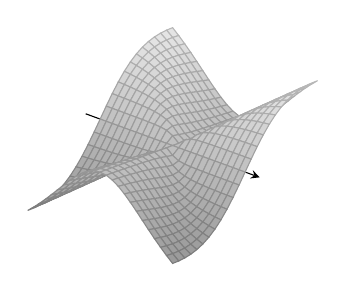
\begin{tikzpicture}[declare function={f(\x,\y)=-\x*(\y)^2/((\x)^2+(\y)^2);}]
  \begin{axis}[view/h=135,width=6cm,axis lines=center,domain=-2:2,domain y=-2:2,colormap={kgray}{gray(0.2cm)=(0.6);gray(1cm)=(0.9);},xtick={\empty},ytick={\empty},ztick={\empty},enlargelimits=true]
%\addplot3[contour gnuplot={output point meta=rawz,number=20,labels=false,},samples=41,z filter/.code=\def\pgfmathresult{-1.6},]{f(x,y)};
 \addplot3[surf,samples=25]{f(x,y)};
%\addplot3[contour gnuplot={draw color = red,levels={0.1,0.2,0.4}}]{f(x,y)};
\end{axis}
\end{tikzpicture}
\caption{}
\label{شکل_سوال_کثیرالمتغیر_ب}
\end{minipage}\hfill
\begin{minipage}{0.3\textwidth}
\centering
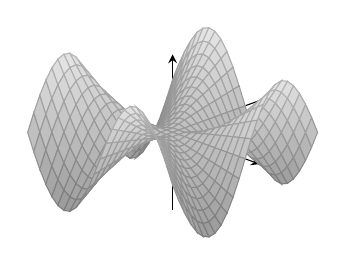
\begin{tikzpicture}[declare function={f(\x,\y)=\x*\y*((\x)^2-(\y)^2)/((\x)^2+(\y)^2);}]
  \begin{axis}[view/h=135,width=6cm,axis lines=center,domain=-2:2,domain y=-2:2,colormap={kgray}{gray(0.2cm)=(0.6);gray(1cm)=(0.9);},xtick={\empty},ytick={\empty},ztick={\empty},enlargelimits=true]
%\addplot3[contour gnuplot={output point meta=rawz,number=20,labels=false,},samples=41,z filter/.code=\def\pgfmathresult{-1.6},]{f(x,y)};
 \addplot3[surf,samples=25]{f(x,y)};
%\addplot3[contour gnuplot={draw color = red,levels={0.1,0.2,0.4}}]{f(x,y)};
\end{axis}
\end{tikzpicture}
\caption{}
\label{شکل_سوال_کثیرالمتغیر_ہ}
\end{minipage}\hfill
\begin{minipage}{0.3\textwidth}
\centering
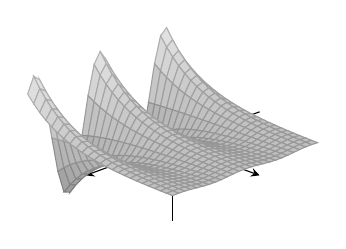
\begin{tikzpicture}[declare function={f(\x,\y)=e^(-\y)*cos(deg(\x));}]
  \begin{axis}[view/h=135,width=6cm,axis lines=center,domain=-7:7,domain y=-2:2,colormap={kgray}{gray(0.2cm)=(0.6);gray(1cm)=(0.9);},xtick={\empty},ytick={\empty},ztick={\empty},enlargelimits=true]
%\addplot3[contour gnuplot={output point meta=rawz,number=20,labels=false,},samples=41,z filter/.code=\def\pgfmathresult{-1.6},]{f(x,y)};
 \addplot3[surf,samples=25]{f(x,y)};
%\addplot3[contour gnuplot={draw color = red,levels={0.1,0.2,0.4}}]{f(x,y)};
\end{axis}
\end{tikzpicture}
\caption{}
\label{شکل_سوال_کثیرالمتغیر_د}
\end{minipage}
\begin{minipage}{0.3\textwidth}
\centering
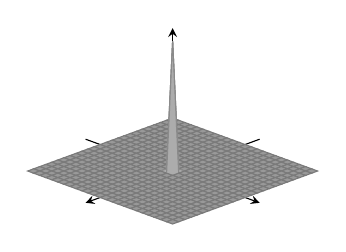
\begin{tikzpicture}[declare function={f(\x,\y)=1/(4*(\x)^2+(\y)^2);}]
  \begin{axis}[view/h=135,width=6cm,axis lines=center,domain=-2:2,domain y=-2:2,colormap={kgray}{gray(0.2cm)=(0.6);gray(1cm)=(0.9);},xtick={\empty},ytick={\empty},ztick={\empty},enlargelimits=true]
%\addplot3[contour gnuplot={output point meta=rawz,number=20,labels=false,},samples=41,z filter/.code=\def\pgfmathresult{-1.6},]{f(x,y)};
 \addplot3[surf,samples=25]{f(x,y)};
%\addplot3[contour gnuplot={draw color = red,levels={0.1,0.2,0.4}}]{f(x,y)};
\end{axis}
\end{tikzpicture}
\caption{}
\label{شکل_سوال_کثیرالمتغیر_ج}
\end{minipage}\hfill
\begin{minipage}{0.3\textwidth}
\centering
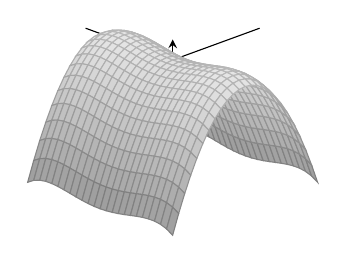
\begin{tikzpicture}[declare function={f(\x,\y)=(\y)^2-(\y)^4-(\x)^2;}]
  \begin{axis}[view/h=135,width=6cm,axis lines=center,domain=-2:2,domain y=-1:1,colormap={kgray}{gray(0.2cm)=(0.6);gray(1cm)=(0.9);},xtick={\empty},ytick={\empty},ztick={\empty},enlargelimits=true]
%\addplot3[contour gnuplot={output point meta=rawz,number=20,labels=false,},samples=41,z filter/.code=\def\pgfmathresult{-1.6},]{f(x,y)};
 \addplot3[surf,samples=25]{f(x,y)};
%\addplot3[contour gnuplot={draw color = red,levels={0.1,0.2,0.4}}]{f(x,y)};
\end{axis}
\end{tikzpicture}
\caption{}
\label{شکل_سوال_کثیرالمتغیر_و}
\end{minipage}\hfill
\begin{minipage}{0.3\textwidth}
\centering
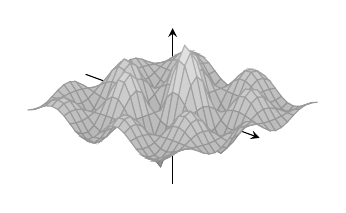
\begin{tikzpicture}[declare function={f(\x,\y)=cos(deg(\x))*sin(deg(\y))*e^(-1/4*sqrt((\x)^2+(\y)^2));}]
  \begin{axis}[view/h=135,width=6cm,axis lines=center,domain=-7:7,domain y=-7:7,colormap={kgray}{gray(0.2cm)=(0.6);gray(1cm)=(0.9);},xtick={\empty},ytick={\empty},ztick={\empty},enlargelimits=true]
%\addplot3[contour gnuplot={output point meta=rawz,number=20,labels=false,},samples=41,z filter/.code=\def\pgfmathresult{-1.6},]{f(x,y)};
 \addplot3[surf,samples=25]{f(x,y)};
%\addplot3[contour gnuplot={draw color = red,levels={0.1,0.2,0.4}}]{f(x,y)};
\end{axis}
\end{tikzpicture}
\caption{}
\label{شکل_سوال_کثیرالمتغیر_الف}
\end{minipage}
\end{figure}

%=====================
\موٹا{دو متغیرات کے تفاعل کی پہچان}\\
سوال \حوالہ{سوال_کثیرالمتغیر_ہم_قد_منحنیات_الف} تا سوال \حوالہ{سوال_کثیرالمتغیر_ہم_قد_منحنیات_ب} میں تفاعل کی قیمتوں کو دو طرح دکھائیں۔ (ا)  سطح \عددی{z=f(x,y)} کو ترسیم کرتے ہوئے اور (ب) تفاعل کے دائرہ کار میں منتخب ہم قد منحنیات ترسیم کرتے ہوئے۔ ہر ایک  ہم قد  منحنی  کی نشاندہی  تفاعل کی قیمت سے کریں۔  

\ابتدا{سوال}\شناخت{سوال_کثیرالمتغیر_ہم_قد_منحنیات_الف}
$f(x,y)=y^2$
\ابتدا{جواب}
\wf{\unexpanded{
\begin{minipage}{0.45\textwidth}
\centering
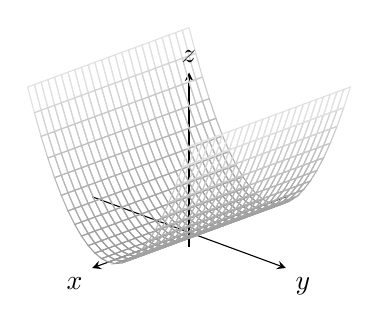
\begin{tikzpicture}[declare function={f(\x,\y)=(\y)^2;}]
  \begin{axis}[view/h=135,small,axis lines=center,domain=-1:1,domain y=-1:1,colormap={kgray}{gray(0.2cm)=(0.6);gray(1cm)=(0.9);},xtick={\empty},ytick={\empty},ztick={\empty},enlargelimits=true,xlabel={$x$},ylabel={$y$},zlabel={$z$},xlabel style={anchor=north east},ylabel style={anchor=north west},zlabel style={anchor=south}]
%\addplot3[, contour gnuplot={output point meta=rawz,number=4,labels=false,},samples=41,z filter/.code=\def\pgfmathresult{-1.6},]{f(x,y)};
 \addplot3[mesh,samples=25]{f(x,y)};
%\addplot3[, contour gnuplot={draw color = red,levels={0.1,0.2,0.4}}]{f(x,y)};
\end{axis}
\end{tikzpicture}
\end{minipage}\hfill
\begin{minipage}{0.45\textwidth}
\centering
\begin{tikzpicture}[declare function={f(\x,\y)=(\y)^2;}]
  \begin{axis}[view/h=135,small,axis lines=center,domain=-1:1,domain y=-1:1,colormap={kgray}{gray(0.2cm)=(0.6);gray(1cm)=(0.9);},xtick={\empty},ytick={\empty},ztick={\empty},enlargelimits=true,hide z axis,,xlabel={$x$},ylabel={$y$},zlabel={$z$},xlabel style={anchor=north east},ylabel style={anchor=north west},zlabel style={anchor=south},colormap={kdark}{gray(0.2cm)=(0.2);gray(1cm)=(0.2);}]
\addplot3[, contour gnuplot={output point meta=rawz,number=4,labels=true,},samples=41,z filter/.code=\def\pgfmathresult{0},]{f(x,y)};
 %\addplot3[mesh,samples=25]{f(x,y)};
%\addplot3[, contour gnuplot={draw color = red,levels={0.1,0.2,0.4}}]{f(x,y)};
\end{axis}
\end{tikzpicture}
\end{minipage}
}}
\انتہا{جواب}
\انتہا{سوال}
%===================
\ابتدا{سوال}
$f(x,y)=4-y^2$
\انتہا{سوال}
%===================
\ابتدا{سوال}
$f(x,y)=x^2+y^2$
\ابتدا{جواب}
\wf{\unexpanded{
\begin{minipage}{0.45\textwidth}
\centering
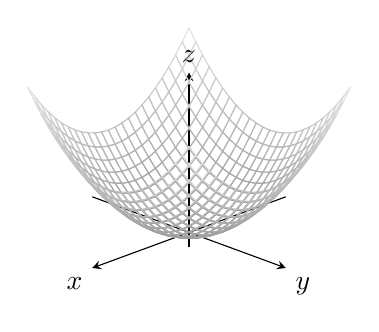
\begin{tikzpicture}[declare function={f(\x,\y)=(\x)^2+(\y)^2;}]
  \begin{axis}[view/h=135,small,axis lines=center,domain=-1:1,domain y=-1:1,colormap={kgray}{gray(0.2cm)=(0.6);gray(1cm)=(0.9);},xtick={\empty},ytick={\empty},ztick={\empty},enlargelimits=true,xlabel={$x$},ylabel={$y$},zlabel={$z$},xlabel style={anchor=north east},ylabel style={anchor=north west},zlabel style={anchor=south}]
%\addplot3[, contour gnuplot={output point meta=rawz,number=4,labels=false,},samples=41,z filter/.code=\def\pgfmathresult{-1.6},]{f(x,y)};
 \addplot3[mesh,samples=25]{f(x,y)};
%\addplot3[, contour gnuplot={draw color = red,levels={0.1,0.2,0.4}}]{f(x,y)};
\end{axis}
\end{tikzpicture}
\end{minipage}\hfill
\begin{minipage}{0.45\textwidth}
\centering
\begin{tikzpicture}[declare function={f(\x,\y)=(\x)^2+(\y)^2;}]
  \begin{axis}[view/h=135,small,axis lines=center,domain=-1:1,domain y=-1:1,colormap={kgray}{gray(0.2cm)=(0.6);gray(1cm)=(0.9);},xtick={\empty},ytick={\empty},ztick={\empty},enlargelimits=true,hide z axis,xlabel={$x$},ylabel={$y$},zlabel={$z$},xlabel style={anchor=north east},ylabel style={anchor=north west},zlabel style={anchor=south},colormap={kdark}{gray(0.2cm)=(0.2);gray(1cm)=(0.2);}]
\addplot3[, contour gnuplot={output point meta=rawz,number=4,labels=true,},samples=41,z filter/.code=\def\pgfmathresult{0},]{f(x,y)};
 %\addplot3[mesh,samples=25]{f(x,y)};
%\addplot3[, contour gnuplot={draw color = red,levels={0.1,0.2,0.4}}]{f(x,y)};
\end{axis}
\end{tikzpicture}
\end{minipage}
}}
\انتہا{جواب}
\انتہا{سوال}
%===================
\ابتدا{سوال}
$f(x,y)=\sqrt{x^2+y^2}$
\انتہا{سوال}
%===================
\ابتدا{سوال}
$f(x,y)=-(x^2+y^2)$
\ابتدا{جواب}
\wf{\unexpanded{
\begin{minipage}{0.45\textwidth}
\centering
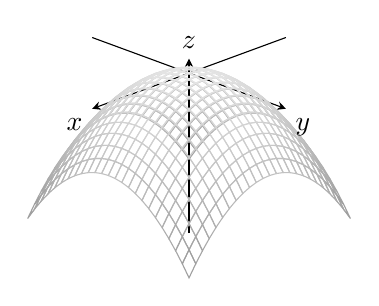
\begin{tikzpicture}[declare function={f(\x,\y)=-(\x)^2-(\y)^2;}]
  \begin{axis}[view/h=135,small,axis lines=center,domain=-1:1,domain y=-1:1,colormap={kgray}{gray(0.2cm)=(0.6);gray(1cm)=(0.9);},xtick={\empty},ytick={\empty},ztick={\empty},enlargelimits=true,xlabel={$x$},ylabel={$y$},zlabel={$z$},xlabel style={anchor=north east},ylabel style={anchor=north west},zlabel style={anchor=south}]
%\addplot3[, contour gnuplot={output point meta=rawz,number=4,labels=false,},samples=41,z filter/.code=\def\pgfmathresult{-1.6},]{f(x,y)};
 \addplot3[mesh,samples=25]{f(x,y)};
%\addplot3[, contour gnuplot={draw color = red,levels={0.1,0.2,0.4}}]{f(x,y)};
\end{axis}
\end{tikzpicture}
\end{minipage}\hfill
\begin{minipage}{0.45\textwidth}
\centering
\begin{tikzpicture}[declare function={f(\x,\y)=-(\x)^2-(\y)^2;}]
  \begin{axis}[view/h=135,width=6cm,axis lines=center,domain=-1:1,domain y=-1:1,colormap={kgray}{gray(0.2cm)=(0.6);gray(1cm)=(0.9);},xtick={\empty},ytick={\empty},ztick={\empty},enlargelimits=true,hide z axis,xlabel={$x$},ylabel={$y$},zlabel={$z$},xlabel style={anchor=north east},ylabel style={anchor=north west},zlabel style={anchor=south},colormap={kdark}{gray(0.2cm)=(0.2);gray(1cm)=(0.2);}]
\addplot3[, contour gnuplot={output point meta=rawz,number=4,labels=true,},samples=41,z filter/.code=\def\pgfmathresult{0},]{f(x,y)};
 %\addplot3[mesh,samples=25]{f(x,y)};
%\addplot3[, contour gnuplot={draw color = red,levels={0.1,0.2,0.4}}]{f(x,y)};
\end{axis}
\end{tikzpicture}
\end{minipage}
}}
\انتہا{جواب}
\انتہا{سوال}
%===================
\ابتدا{سوال}
$f(x,y)=4-x^2-y^2$
\انتہا{سوال}
%===================
\ابتدا{سوال}
$f(x,y)=4x^2+y^2$
\ابتدا{جواب}
\wf{\unexpanded{
\begin{minipage}{0.45\textwidth}
\centering
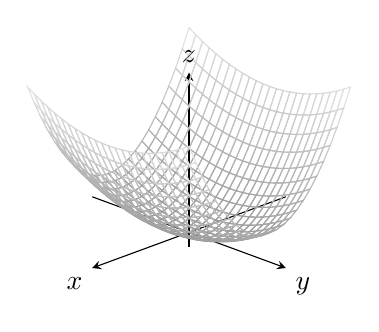
\begin{tikzpicture}[declare function={f(\x,\y)=4*(\x)^2+(\y)^2;}]
  \begin{axis}[view/h=135,small,axis lines=center,domain=-1:1,domain y=-1:1,colormap={kgray}{gray(0.2cm)=(0.6);gray(1cm)=(0.9);},xtick={\empty},ytick={\empty},ztick={\empty},enlargelimits=true,xlabel={$x$},ylabel={$y$},zlabel={$z$},xlabel style={anchor=north east},ylabel style={anchor=north west},zlabel style={anchor=south}]
%\addplot3[, contour gnuplot={output point meta=rawz,number=4,labels=false,},samples=41,z filter/.code=\def\pgfmathresult{-1.6},]{f(x,y)};
 \addplot3[mesh,samples=25]{f(x,y)};
%\addplot3[, contour gnuplot={draw color = red,levels={0.1,0.2,0.4}}]{f(x,y)};
\end{axis}
\end{tikzpicture}
\end{minipage}\hfill
\begin{minipage}{0.45\textwidth}
\centering
\begin{tikzpicture}[declare function={f(\x,\y)=4*(\x)^2+(\y)^2;}]
  \begin{axis}[view/h=135,small,axis lines=center,domain=-1:1,domain y=-1:1,colormap={kgray}{gray(0.2cm)=(0.6);gray(1cm)=(0.9);},xtick={\empty},ytick={\empty},ztick={\empty},enlargelimits=true,hide z axis,xlabel={$x$},ylabel={$y$},zlabel={$z$},xlabel style={anchor=north east},ylabel style={anchor=north west},zlabel style={anchor=south},colormap={kdark}{gray(0.2cm)=(0.2);gray(1cm)=(0.2);}]
\addplot3[, contour gnuplot={output point meta=rawz,number=4,labels=true,},samples=41,z filter/.code=\def\pgfmathresult{0},]{f(x,y)};
 %\addplot3[mesh,samples=25]{f(x,y)};
%\addplot3[, contour gnuplot={draw color = red,levels={0.1,0.2,0.4}}]{f(x,y)};
\end{axis}
\end{tikzpicture}
\end{minipage}
}}
\انتہا{جواب}
\انتہا{سوال}
%===================
\ابتدا{سوال}
$f(x,y)=4x^2+y^2+1$
\انتہا{سوال}
%===================
\ابتدا{سوال}
$f(x,y)=1-\abs{y}$
\ابتدا{جواب}
\wf{\unexpanded{
\begin{minipage}{0.45\textwidth}
\centering
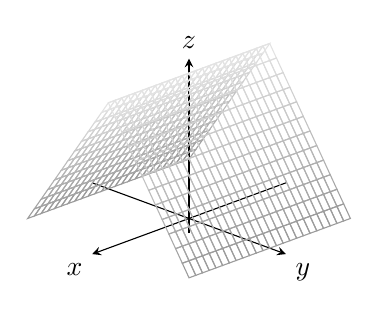
\begin{tikzpicture}[declare function={f(\x,\y)=1-abs(\y);}]
  \begin{axis}[view/h=135,small,axis lines=center,domain=-1:1,domain y=-1:1,colormap={kgray}{gray(0.2cm)=(0.6);gray(1cm)=(0.9);},xtick={\empty},ytick={\empty},ztick={\empty},enlargelimits=true,xlabel={$x$},ylabel={$y$},zlabel={$z$},xlabel style={anchor=north east},ylabel style={anchor=north west},zlabel style={anchor=south}]
%\addplot3[, contour gnuplot={output point meta=rawz,number=4,labels=false,},samples=41,z filter/.code=\def\pgfmathresult{-1.6},]{f(x,y)};
 \addplot3[mesh,samples=25]{f(x,y)};
%\addplot3[, contour gnuplot={draw color = red,levels={0.1,0.2,0.4}}]{f(x,y)};
\end{axis}
\end{tikzpicture}
\end{minipage}\hfill
\begin{minipage}{0.45\textwidth}
\centering
\begin{tikzpicture}[declare function={f(\x,\y)=1-abs(\y);}]
  \begin{axis}[view/h=135,small,axis lines=center,domain=-1:1,domain y=-1:1,colormap={kgray}{gray(0.2cm)=(0.6);gray(1cm)=(0.9);},xtick={\empty},ytick={\empty},ztick={\empty},enlargelimits=true,hide z axis,xlabel={$x$},ylabel={$y$},zlabel={$z$},xlabel style={anchor=north east},ylabel style={anchor=north west},zlabel style={anchor=south},colormap={kdark}{gray(0.2cm)=(0.2);gray(1cm)=(0.2);}]
\addplot3[, contour gnuplot={output point meta=rawz,number=4,labels=true,},samples=41,z filter/.code=\def\pgfmathresult{0},]{f(x,y)};
 %\addplot3[mesh,samples=25]{f(x,y)};
%\addplot3[, contour gnuplot={draw color = red,levels={0.1,0.2,0.4}}]{f(x,y)};
\end{axis}
\end{tikzpicture}
\end{minipage}
}}
\انتہا{جواب}
\انتہا{سوال}
%===================
\ابتدا{سوال}\شناخت{سوال_کثیرالمتغیر_ہم_قد_منحنیات_ب}
$f(x,y)=1-\abs{x}-\abs{y}$
\انتہا{سوال}
%===================

\موٹا{ہم قد سطحیں}\\
سوال \حوالہ{سوال_کثیر_المتغیر_ہم_قد_سطح_الف} تا سوال \حوالہ{سوال_کثیر_المتغیر_ہم_قد_سطح_ب} میں تفاعل کا  ایک علامتی  ہم قد سطح  کا خاکہ بنائیں۔

\ابتدا{سوال}\شناخت{سوال_کثیر_المتغیر_ہم_قد_سطح_الف}
$f(x,y,z)=x^2+y^2+z^2$
\ابتدا{جواب}
\wf{\unexpanded{
\begin{center}
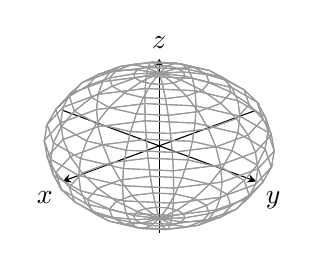
\begin{tikzpicture}[declare function={fx(\x,\y)=sin(\x)*cos(\y);fy(\x,\y)=sin(\x)*sin(\y);fz(\x,\y)=cos(\x);}]
  \begin{axis}[view/h=135,small,axis lines=center,domain=0:180,domain y=0:360,colormap={kgray}{gray(0.2cm)=(0.6);gray(1cm)=(0.6);},xtick={\empty},ytick={\empty},ztick={\empty},enlargelimits=true,xlabel={$x$},ylabel={$y$},zlabel={$z$},xlabel style={anchor=north east},ylabel style={anchor=north west},zlabel style={anchor=south}]
%\addplot3[, contour gnuplot={output point meta=rawz,number=4,labels=false,},samples=41,z filter/.code=\def\pgfmathresult{0},]{f(x,y)};
 \addplot3[mesh,samples=15]({fx(x,y)},{fy(x,y)},{fz(x,y)});
%\addplot3[, contour gnuplot={draw color = red,levels={0.1,0.2,0.4}}]({fx(x,y)},{fy(x,y)},{fz(x,y)});
\end{axis}
\end{tikzpicture}
\end{center}
$f(x,y,z)=x^2+y^2+z^2=1$
}}
\انتہا{جواب}
\انتہا{سوال}
%==================
\ابتدا{سوال}
$f(x,y,z)=\ln(x^2+y^2+z^2)$
\انتہا{سوال}
%================
\ابتدا{سوال}
$f(x,y,z)=x+z$
\ابتدا{جواب}
\wf{\unexpanded{
\begin{center}
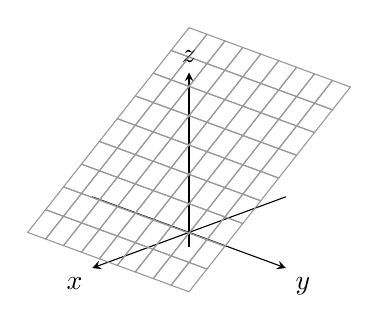
\begin{tikzpicture}[declare function={f(\x,\y)=1-\x;}]
  \begin{axis}[view/h=135,small,axis lines=center,domain=-1:1,domain y=-1:1,colormap={kgray}{gray(0.2cm)=(0.6);gray(1cm)=(0.6);},xtick={\empty},ytick={\empty},ztick={\empty},enlargelimits=true,xlabel={$x$},ylabel={$y$},zlabel={$z$},xlabel style={anchor=north east},ylabel style={anchor=north west},zlabel style={anchor=south}]
%\addplot3[, contour gnuplot={output point meta=rawz,number=4,labels=false,},samples=41,z filter/.code=\def\pgfmathresult{0},]{f(x,y)};
 \addplot3[mesh,samples=10]{f(x,y)};
%\addplot3[, contour gnuplot={draw color = red,levels={0.1,0.2,0.4}}]{f(x,y)};
\end{axis}
\end{tikzpicture}
\end{center}
$f(x,y,z)=x+z=1$
}}
\انتہا{جواب}
\انتہا{سوال}
%================
\ابتدا{سوال}
$f(x,y,z)=z$
\انتہا{سوال}
%================
\ابتدا{سوال}
$f(x,y,z)=x^2+y^2$
\ابتدا{جواب}
\wf{\unexpanded{
\begin{center}
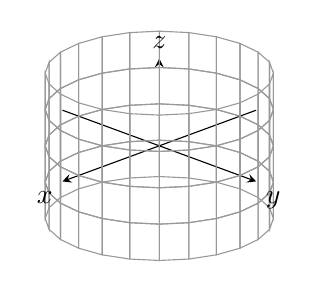
\begin{tikzpicture}[declare function={fx(\x,\y)=cos(\x);fy(\x,\y)=sin(\x);fz(\x,\y)=\y;}]
  \begin{axis}[view/h=135,small,axis lines=center,domain=0:360,domain y=-1:1,colormap={kgray}{gray(0.2cm)=(0.6);gray(1cm)=(0.6);},xtick={\empty},ytick={\empty},ztick={\empty},enlargelimits=true,xlabel={$x$},ylabel={$y$},zlabel={$z$},xlabel style={anchor=north east},ylabel style={anchor=north west},zlabel style={anchor=south}]
%\addplot3[, contour gnuplot={output point meta=rawz,number=4,labels=false,},samples=41,z filter/.code=\def\pgfmathresult{0},]{f(x,y)};
 \addplot3[smooth,mesh,samples=25,samples y=5]({fx(x,y)},{fy(x,y)},{fz(x,y)});
%\addplot3[, contour gnuplot={draw color = red,levels={0.1,0.2,0.4}}]({fx(x,y)},{fy(x,y)},{fz(x,y)});
\end{axis}
\end{tikzpicture}
\end{center}
$f(x,y,z)=x^2+y^2=1$
}}
\انتہا{جواب}
\انتہا{سوال}
%================
\ابتدا{سوال}
$f(x,y,z)=y^2+z^2$
\انتہا{سوال}
%================
\ابتدا{سوال}
$f(x,y,z)=z-x^2-y^2$
\ابتدا{جواب}
\wf{\unexpanded{
\begin{center}
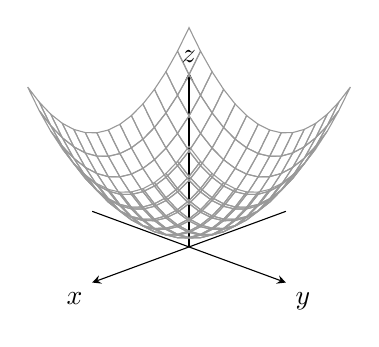
\begin{tikzpicture}[declare function={f(\x,\y)=1+(\x)^2+(\y)^2;}]
  \begin{axis}[view/h=135,small,axis lines=center,domain=-1:1,domain y=-1:1,colormap={kgray}{gray(0.2cm)=(0.6);gray(1cm)=(0.6);},xtick={\empty},ytick={\empty},ztick={\empty},enlargelimits=true,xlabel={$x$},ylabel={$y$},zlabel={$z$},xlabel style={anchor=north east},ylabel style={anchor=north west},zlabel style={anchor=south}]
%\addplot3[, contour gnuplot={output point meta=rawz,number=4,labels=false,},samples=41,z filter/.code=\def\pgfmathresult{0},]{f(x,y)};
 \addplot3[mesh,samples=15]{f(x,y)};
%\addplot3[, contour gnuplot={draw color = red,levels={0.1,0.2,0.4}}]{f(x,y)};
\end{axis}
\end{tikzpicture}
\end{center}
$f(x,y,z)=z-x^2-y^2=1$\\
یعنی
$z=x^2+y^2+1$
}}
\انتہا{جواب}
\انتہا{سوال}
%================
\ابتدا{سوال}\شناخت{سوال_کثیر_المتغیر_ہم_قد_سطح_ب}
$f(x,y,z)=\tfrac{x^2}{25}+\tfrac{y^2}{16}+\tfrac{z^2}{9}$
\انتہا{سوال}
%================
\موٹا{ہم قد منحنی کی  تلاش}\\
سوال \حوالہ{سوال_کثیر_المتغیر_ہم_قد_منحنی_تلاش_الف} تا سوال \حوالہ{سوال_کثیر_المتغیر_ہم_قد_منحنی_تلاش_ب} میں  تفاعل \عددی{f(x,y)} کی اس  ہم قد منحنی کی مساوات تلاش کریں جو  دیے گئے نقطہ سے گزرتی  ہو۔

\ابتدا{سوال}\شناخت{سوال_کثیر_المتغیر_ہم_قد_منحنی_تلاش_الف}
$f(x,y)=16-x^2-y^2,\quad (2\sqrt{2},\sqrt{2})$
\ابتدا{جواب}
\wf{\unexpanded{
$x^2+y^2=10$
}}
\انتہا{جواب}
\انتہا{سوال}
%================
\ابتدا{سوال}
$f(x,y)=\sqrt{x^2-1},\quad (1,0)$
\انتہا{سوال}
%================
\ابتدا{سوال}
$f(x,y)=\int\limits_x^y\frac{\dif t}{1+t^2},\quad (-\sqrt{2},\sqrt{2})$
\ابتدا{جواب}
\wf{\unexpanded{
$\tan^{-1}y-\tan^{-1}x=2\tan^{-1}\sqrt{2}$
}}
\انتہا{جواب}
\انتہا{سوال}
%================
\ابتدا{سوال}\شناخت{سوال_کثیر_المتغیر_ہم_قد_منحنی_تلاش_ب}
$f(x,y)=\sum\limits_{n=0}^{\infty}\big(\frac{x}{y}\big)^n,\quad (1,2)$
\انتہا{سوال}
%================
\موٹا{ہم قد سطح کی تلاش}\\
سوال \حوالہ{سوال_کثیر_المتغیر_ہم_قد_سطح_تلاش_الف} تا سوال \حوالہ{سوال_کثیر_المتغیر_ہم_قد_سطح_تلاش_ب} میں دیے گئے نقطہ سے گزرتی ہم قد سطح کی مساوات تلاش کریں۔

\ابتدا{سوال}\شناخت{سوال_کثیر_المتغیر_ہم_قد_سطح_تلاش_الف}
$f(x,y,z)=\sqrt{x-y}-\ln z,\quad (3,-1,1)$
\ابتدا{جواب}
\wf{\unexpanded{
$\sqrt{x-y}-\ln z=2$
}}
\انتہا{جواب}
\انتہا{سوال}
%=================
\ابتدا{سوال}
$f(x,y,z)=\ln(x^2+y+z^2),\quad (-1,2,1)$
\انتہا{سوال}
%==================
\ابتدا{سوال}
$g(x,y,z)=\sum\limits_{n=0}^{\infty}\frac{(x+y)^n}{n!z^n},\quad (\ln 2,\ln 4,3)$
\ابتدا{جواب}
\wf{\unexpanded{
$\tfrac{x+y}{z}=\ln 2$
}}
\انتہا{جواب}
\انتہا{سوال}
%==================
\ابتدا{سوال}\شناخت{سوال_کثیر_المتغیر_ہم_قد_سطح_تلاش_ب}
$g(x,y,z)=\int\limits_x^y\frac{\dif \theta}{\sqrt{1-\theta^2}}+\int\limits_{\sqrt{2}}^{z}\frac{\dif t}{t\sqrt{t^2-1}},\quad (0,\tfrac{1}{2},2)$
\انتہا{سوال}
%==================

\موٹا{نظریہ اور مثالیں}\\
\ابتدا{سوال}\ترچھا{فضا میں ایک لکیر پر تفاعل کی زیادہ سے زیادہ قیمت۔}\\
کیا لکیر \عددی{x=20-t,\,y=t,\,z=20} پر تفاعل \عددی{f(x,y,z)=xyz} کی  زیادہ سے زیادہ قیمت پائی جاتی ہے؟ اگر  ہو، تب اس کی قیمت کتنی ہو گی؟ اپنے جواب کی وجہ پیش کریں۔ (اشارہ:اس لکیر پر \عددی{w=(f,y,z)} متغیر \عددی{t} کا قابل تفرق تفاعل ہے۔)
\ابتدا{جواب}
\wf{\unexpanded{
جی ہاں، \عددی{2000}
}}
\انتہا{جواب}
\انتہا{سوال}
%==============
\ابتدا{سوال}\ترچھا{فضا میں ایک لکیر پر تفاعل کی کم سے کم  قیمت۔}\\
کیا لکیر \عددی{x=t-1,\,y=t-2,\,z=t+7} پر تفاعل \عددی{f(x,y,z)=xy-z} کی کم سے کم  قیمت پائی جاتی ہے؟ اگر  ہو، تب اس کی قیمت کتنی ہو گی؟ اپنے جواب کی وجہ پیش کریں۔ (اشارہ:اس لکیر پر \عددی{w=(f,y,z)} متغیر \عددی{t} کا قابل تفرق تفاعل ہے۔)
\انتہا{سوال}
%=================
\ابتدا{سوال}\ترچھا{جہاز کا صوتی دھماکا}\\
ایک جہاز کے نیچے زمین پر اس خطہ کی چوڑائی \عددی{w}  جہاں  جہاز کا   صوتی دھماکا   انسان  برائے راست (جو   فضا میں ہوا کی مختلف  سطحوں سے منعکس نہ ہو)  سن سکتا ہو  ، درج ذیل کا  تفاعل ہو گا۔
\begin{itemize}
\item
\عددی{T} زمین پر ہوا کی  درجہ حرارت (کیلون) 
\item
\عددی{h} جہاز کی بلندی (کلو میٹر)
\item
\عددی{d}  درجہ حرارت کی انتصابی  شرح تبدیلی (کیلون فی کلومیٹر)
\end{itemize}
اس چوڑائی کا  کلیہ درج ذیل ہے۔
\begin{align*}
w=4\sqrt{\tfrac{Th}{d}}
\end{align*}
یہ جہاز \عددی{\SI{16.8}{\kilo\meter}} کی بلندی پر پرواز کرتا ہوا  بحیرہ عرب  سے کراچی  شہر    پہنچ رہا ہے۔ اگر سطحی درجہ حرارت \عددی{\SI{290}{\kelvin}} اور انتصابی شرح حرارت \عددی{\SI{5}{\kelvin\per\kilo\meter}} ہو تب   جہاز ساحل سے کتنا دور ہو گا جب اس کا صوتی دھماکا سنائی دے۔
\ابتدا{جواب}
\wf{\unexpanded{
$\SI{63}{\kilo\meter}$
}}
\انتہا{جواب}
\انتہا{سوال}
%================
\ابتدا{سوال}
جیسا کہ آپ جانتے ہیں، واحد حقیقی متغیر کے حقیقی قیمت تفاعل کی ترسیم دو محددی فضا کا سلسلہ ہو تا ہے۔ دو غیر تابع حقیقی متغیرات کے حقیقی قیمت تفاعل  کی ترسیم تین محددی فضا کا سلسلہ ہوتا ہے۔    تین غیر تابع حقیقی متغیرات کے حقیقی قیمت تفاعل  کی ترسیم چار  محددی فضا کا سلسلہ ہوتا ہے۔   آپ چار غیر تابع متغیرات کے تفاعل \عددی{f(x_1,x_2,x_3,x_4)}  کی ترسیم کے بارے میں کیا کہیں گے؟ ۔   آپ \عددی{n}  غیر تابع متغیرات کے تفاعل \عددی{f(x_1,x_2,x_3,\cdots,x_n)}  کی ترسیم کے بارے میں کیا کہیں گے؟
\انتہا{سوال}
%==========
\موٹا{کمپیوٹر کا استعمال۔صریح سطح}\\
کمپیوٹر استعمال کرتے ہوئے سوال \حوالہ{سوال_کثیرالمتغیر_صریح_سطح_الف} تا سوال \حوالہ{سوال_کثیرالمتغیر_صریح_سطح_ب} میں درج ذیل اقدام کریں۔
\begin{enumerate}[a.]
\item
دیے گئے مستطیل پر سطح ترسیم کریں۔
\item
اس مستطیل میں کئی ہم قد منحنیات ترسیم کریں۔
\item
دیے گئے نقطہ سے گزرتی  ہوئی   \عددی{f} کی   ہم قد منحنی ترسیم کریں۔ 
\end{enumerate}

\ابتدا{سوال}\شناخت{سوال_کثیرالمتغیر_صریح_سطح_الف}
$f(x,y)=x\sin\tfrac{y}{2}+y\sin 2x,\quad 0\le x\le 5\pi,\quad 0\le y\le 5\pi$
\انتہا{سوال}
%=================
\ابتدا{سوال}
$f(x,y)=(\sin x)(\cos x)e^{\sqrt{x^2+y^2}/8},\quad 0\le x\le 5\pi,\quad 0\le y\le 5\pi$
\انتہا{سوال}
%==================
\ابتدا{سوال}
$f(x,y)=\sin(x+2\cos y),\quad -2\pi\le x\le 2\pi,\quad -2\pi\le y\le 2\pi$
\انتہا{سوال}
%==================
\ابتدا{سوال}\شناخت{سوال_کثیرالمتغیر_صریح_سطح_ب}
$f(x,y)=e^{(x^{0.1}-y)}\sin (x^2+y^2),\quad 0\le x\le 2\pi,\quad -2\pi\le y\le \pi$
\انتہا{سوال}
%==================
\موٹا{کمپیوٹر کا استعمال۔خفی  سطح}\\
سوال \حوالہ{سوال_کثیرالمتغیر_ہم_قد_سطحیں_ترسیم_الف} تا سوال \حوالہ{سوال_کثیرالمتغیر_ہم_قد_سطحیں_ترسیم_ب} میں کمپیوٹر استعمال کرتے ہوئے ہم قد سطحیں  ترسیم کریں۔

\ابتدا{سوال}\شناخت{سوال_کثیرالمتغیر_ہم_قد_سطحیں_ترسیم_الف}
$4\ln(x^2+y^2+z^2)=1$
\انتہا{سوال}
%================
\ابتدا{سوال}
$x^2+z^2=1$
\انتہا{سوال}
%=====================
\ابتدا{سوال}
$x+y^2-3z^2=1$
\انتہا{سوال}
%=====================
\ابتدا{سوال}\شناخت{سوال_کثیرالمتغیر_ہم_قد_سطحیں_ترسیم_ب}
$\sin\big(\frac{x}{2}\big)-(\cos y)\sqrt{x^2+z^2}=2$
\انتہا{سوال}
%=====================
\موٹا{کمپیوٹر کا استعمال۔مقدار معلوم   سطح}\\
جیسا آپ کسی مقدار معلوم وقفہ \عددی{I} پر  مستوی میں منحنیات کو مقدار معلوم مساوات \عددی{x=f(t),\,y=g(t)} کی    روپ میں لکھتے ہیں، آپ بعض اوقات کسی مقدار معلوم مستطیل \عددی{a\le u\le b,\, c\le v\le d}وقفہ  پر  فضا میں سطحوں کو    مقدار معلوم تین مساوات \عددی{x=f(u,v),\,y=g(u,v),\,z=h(u,v)}  کی روپ میں لکھ سکتے ہیں۔کمپیوٹر اس قسم کی مقدار معلوم مساواتوں سے سطح  ترسیم کر سکتا ہے۔سوال \حوالہ{سوال_کثیرالمتغیر_مقدار_معلوم_الف} تا سوال \حوالہ{سوال_کثیرالمتغیر_مقدار_معلوم_ب} میں کمپیوٹر کی مدد سے سطحیں ترسیم کریں۔ساتھ ہی \عددی{xy} مستوی میں چند ہم قد منحنیات ترسیم کریں۔

\ابتدا{سوال}\شناخت{سوال_کثیرالمتغیر_مقدار_معلوم_الف}
$x=u\cos v,\quad y=u\sin v,\quad z=u,\quad 0\le u\le 2,\quad 0\le v\le 2\pi$
\انتہا{سوال}
%===================
\ابتدا{سوال}
$x=u\cos v,\quad y=u\sin v,\quad z=v,\quad 0\le u\le 2,\quad 0\le v\le 2\pi$
\انتہا{سوال}
%===================
\ابتدا{سوال}
$x=(2+\cos u)\cos v,\,y=(2+\cos u)\sin v,\, z=\sin u,$\\
$ 0\le u\le 2\pi,\, 0\le v\le 2\pi$
\انتہا{سوال}
%===================
\ابتدا{سوال}\شناخت{سوال_کثیرالمتغیر_مقدار_معلوم_ب}
$x=2\cos u\cos v,\quad y=2\cos u\sin v,\quad z=2\sin u$\\
$0\le u\le 2\pi,\quad 0\le v\le \pi$
\انتہا{سوال}
%======================
\انتہا{سوالات}




\حصہ{حد اور استمرار}
اس حصہ میں کثیر المتغیر تفاعل کی حد اور استمرار پر غور کیا جائے گا۔

\جزوحصہء{حد}
اگر نقطہ \عددی{(x_0,y_0)} کے قریب   تمام نقاط \عددی{(x,y) } کے لئے تفاعل \عددی{f(x,y)}  کی قیمتیں کسی  مقررہ حقیقی عدد \عددی{L} کے  بہت  زیادہ  قریب ہوں تب ہم کہتے ہیں کہ جیسے جیسے \عددی{(x,y)} نقطہ \عددی{(x_0,y_0)} تک  پہنچنے کی کوشش کرتا ہے، تفاعل \عددی{f} کی قیمت \عددی{L} تک پہنچنے کی کوشش کرتی ہے۔ یہ تعریف، واحد متغیر کے تفاعل کی حد کی تعریف کی مانند ہے۔البتہ، دھیان رہے کہ اگر \عددی{(x_0,y_0)} تفاعل \عددی{f}  کے دائرہ کار  کی اندرون میں پایا جاتا ہو تب \عددی{(x,y)} نقطہ \عددی{(x_0,y_0)} تک کسی بھی رخ سے پہنچنے کی کوشش کر سکتا ہے۔جیسا آپ نیچے  دی گئی   مثالوں میں سے چند  میں دیکھیں گے،  قریب پہنچنے کا رخ بعض اوقات مسئلہ کھڑا کر سکتا ہے۔

\ابتدا{تعریف}
اگر ہر عدد \عددی{\epsilon>0} کے لئے ایسا مطابقتی عدد \عددی{\delta>0} پایا جاتا ہو کہ \عددی{f} کے دائرہ کار میں تمام \عددی{(x,y)} کے لئے 
\begin{align}\label{مساوات_کثیرالمتغیر_تعریف_حد_الف}
0<\sqrt{(x-x_0)^2+(y-y_0)^2}<\delta\implies \abs{f(x,y)-L}<\epsilon
\end{align}
ہو ، تب ہم کہتے ہیں کہ \عددی{(x_0,y_0)} تک  \عددی{(x,y)}    پہنچنے سے \عددی{f(x,y)} کی قیمت \اصطلاح{حد}\فرہنگ{حد}\حاشیہب{limit}\فرہنگ{limit} \عددی{L} تک پہنچتی ہے جس کو ہم درج ذیل لکھتے ہیں۔
\begin{align*}
\lim_{(x,y)\to(x_0,y_0)}f(x,y)=L
\end{align*}
\انتہا{تعریف}
%====================

حد کی تعریف میں \عددی{\delta \sigma} کی شرط  اس کی  معادل ہے  کہ، کسی بھی \عددی{\epsilon>0} کے لئے ایسا مطابقتی \عددی{\delta>0} پایا جاتا ہو کہ تمام \عددی{x} کے لئے درج ذیل ہو۔
\begin{align}\label{مساوات_کثیرالمتغیر_تعریف_حد_ب}
0<\abs{x-x_0}<\delta\quad \text{اور}\quad 0<\abs{y-y_0}<\delta\implies \abs{f(x,y)-L}<\epsilon
\end{align}
یوں حد کی قیمت  تلاش کرتے   ہوئے ہم مستوی میں فاصلوں کی صورت یا محدد میں فرق کی صورت میں سوچ سکتے ہیں۔

حد کی تعریف، تفاعل \عددی{f} کے دائرہ کار کی اندرون  کے ساتھ   سرحدی نقاط \عددی{(x_0,y_0)} کے لئے بھی   کارآمد  ہے۔  بس اتنا ضروری ہے کہ نقطہ \عددی{(x,y)} ہر وقت دائرہ کار کے اندر رہے۔

واحد متغیر کے تفاعل کی طرح  درج ذیل دکھائے جا  سکتے ہیں۔
\begin{gather}
\begin{aligned}\label{مساوات_کثیر_المتغیر_قواعد_حد}
\lim_{(x,y)\to(x_0,y_0)}x&=x_0\\
\lim_{(x,y)\to(x_0,y_0)}y&=y_0\\
\lim_{(x,y)\to(x_0,y_0)}k&=k\quad \text{\RL{\عددی{k} کوئی بھی عدد ہو سکتا ہے}}
\end{aligned}
\end{gather}
یہ بھی دکھایا جا سکتا ہے کہ دو تفاعل کے مجموعہ کا حد، ان تفاعل کے انفرادی حد   (اگر دونوں موجود ہوں)کا مجموعہ ہو گا۔اسی طرح   کے نتائج   فرق، حاصل ضرب، حاصل تقسیم، مستقل مضرب اور طاقت کے لئے بھی دکھائے جا سکتے ہیں۔

\ابتدا{مسئلہ}\شناخت{مسئلہ_کثیر_المتغیر_قواعد_حد}\موٹا{دو متغیرات کے تفاعل کی حد کے خواص}\\
اگر 
\begin{align*}
\lim_{(x,y)\to(x_0,y_0)}f(x,y)=L\quad \text{اور}\quad \lim_{(x,y)\to(x_0,y_0)}g(x,y)=M
\end{align*}
ہوں تب درج ذیل قواعد کارآمد  ہوں گے۔
\begin{description}
\item{قاعدہ مجموعہ:}
$\lim[f(x,y)+g(x,y)]=L+M$
\item{قاعدہ فرق:}
$\lim[f(x,y)-g(x,y)]=L-M$
\item{قاعدہ مستقل مضرب:}
$\lim kf(x,y)=kL$
جہاں \عددی{k} کوئی مستقل ہے۔
\item{قاعدہ حاصل تقسیم:}
$\lim\frac{f(x,y)}{g(x,y)}=\frac{L}{M}$
اگر  \عددی{M\ne 0} ہو۔
\item{قاعدہ طاقت:}
$\lim[f(x,y)]^{m/n}=L^{m/n}$
اگر  \عددی{m} اور \عددی{n}ا عداد صحیح   اور \عددی{L^{m/n}} ایک حقیقی عدد ہو۔
\end{description}
تمام حد \عددی{(x,y)\to (x_0,y_0)} کی صورت میں حاصل کیے جائیں گے اور \عددی{L}، \عددی{M} کا حقیقی اعداد ہونا لازمی ہے۔
\انتہا{مسئلہ}
%==========

 مساوات \حوالہ{مساوات_کثیر_المتغیر_قواعد_حد} پر   مسئلہ \حوالہ{مسئلہ_کثیر_المتغیر_قواعد_حد} کے اطلاق سے ہمیں معلوم ہوتا ہے کہ  \عددی{(x,y)\to(x_0,y_0)} کرتے ہوئے  کثیر رکنی اور ناطق تفاعل کی حد     ہم \عددی{(x_0,y_0)} پر  تفاعل کی قیمت   سے حاصل کرتے  ہیں۔ بس اتنا ضروری  ہے کہ  نقطہ \عددی{(x_0,y_0)} پر تفاعل  معین ہو۔

\ابتدا{مثال}
\begin{align*}
\lim_{(x,y)\to(0,1)}\frac{x-xy+3}{x^2y+5xy-y^3}&=\frac{0-(0)(1)+3}{(0)^2(1)+5(0)(1)-(1)^3}=-3\\
\lim_{(x,y)\to(3,-4)}\sqrt{x^2+y^2}&=\sqrt{(3)^2+(-4)^2}=\sqrt{25}=5
\end{align*}
\انتہا{مثال}
%=================
\ابتدا{مثال}
درج ذیل حاصل کریں۔
\begin{align*}
\lim_{(x,y)\to(0,0)}\frac{x^2-xy}{\sqrt{x}-\sqrt{y}}
\end{align*}
حل:\quad
چونکہ \عددی{(x,y)\to(0,0)} پر نسب نما   \عددی{ 0} کو پہنچتا ہے لہٰذا  ہم  قاعدہ حاصل تقسیم (مسئلہ \حوالہ{مسئلہ_کثیر_المتغیر_قواعد_حد})  استعمال نہیں کر سکتے ہیں۔ البتہ نسب نما اور شمار کنندہ کو \عددی{\sqrt{x}+\sqrt{y}} سے ضرب  دے کر ایسا معادل حاصل تقسیم حاصل ہوتا ہے جس کا حد ہم تلاش کر سکتے ہیں:
\begin{align*}
\lim_{(x,y)\to(0,0)}\frac{x^2-xy}{\sqrt{x}-\sqrt{y}}&=\lim_{(x,y)\to(0,0)}\frac{(x^2-xy)(\sqrt{x}+\sqrt{y})}{(\sqrt{x}-\sqrt{y})(\sqrt{x}+\sqrt{y})}\\
&=\lim_{(x,y)\to(0,0)}\frac{x(x-y)(\sqrt{x}+\sqrt{y})}{x-y}&&\text{الجبرا}\\
&=\lim_{(x,y)\to(0,0)}x(\sqrt{x}+\sqrt{y})&&\text{\RL{جزو \عددی{(x-y)} کاٹا گیا}}\\
&=0(\sqrt{0}+\sqrt{0})=0
\end{align*} 
\انتہا{مثال}
%================

\جزوحصہء{استمرار}
واحد متغیر کے تفاعل کی طرح، استمرار کی تعریف  حد کی صورت میں کی جاتی ہے۔

\ابتدا{تعریف}
اگر 
\begin{enumerate}[a.]
\item
\عددی{(x_0,y_0)} پر \عددی{f} معین ہو،
\item
\عددی{\lim_{(x,y)\to(x_0,y_0)}f(x,y)} موجود ہو،
\item
\عددی{\lim_{(x,y)\to(x_0,y_0)}f(x,y)=f(x_0,y_0)} ہو،
\end{enumerate} 
تب تفاعل  \عددی{f}    \اصطلاح{نقطہ \عددی{(x_0,y_0)} پر استمراری}\فرہنگ{استمراری!نقطہ پر}\حاشیہب{continuous}\فرہنگ{continuous!at a point} ہو گا۔ ایک  تفاعل  جو اپنے دائرہ کار کے  ہر نقطہ پر استمراری ہو\اصطلاح{ استمراری}\فرہنگ{استمراری}\حاشیہب{continuous}\فرہنگ{continuous} ہو گا۔
\انتہا{تعریف}
%===============

حد کی تعریف کی طرح،  استمرار کی تعریف بھی \عددی{f} کے دائرہ کار کے تمام اندرونی نقاط کے ساتھ  ساتھ  سرحدی نقاط پر بھی قابل اطلاق  ہوتا ہے بس اتنا ضروری ہے کہ پورے  وقت  نقطہ \عددی{(x,y)}تفاعل کے دائرہ کار میں رہے۔

جیسا آپ  دیکھ سکتے ہیں، مسئلہ \حوالہ{مسئلہ_کثیر_المتغیر_قواعد_حد}    کا ایک نتیجہ  یہ ہے  کہ استمراری تفاعل  کے الجبرائی  جوڑ  ہر اس نقطہ پر استمراری ہوں گے جس پر تمام شامل تفاعل استمراری ہوں۔اس کا مطلب ہے کہ جہاں  تمام   استمراری تفاعل استمراری ہوں وہاں ان  کے مجموعہ، فرق، حاصل ضرب،  مستقل مضرب، حاصل تقسیم اور طاقت استمراری ہوں گے۔   بالخصوص دو متغیرات کی کثیر رکنی اور ناطق تفاعل ان تمام نقطوں پر استمراری ہوں گے جہاں یہ معین ہوں۔

اگر  \عددی{x} اور \عددی{y} کا استمراری تفاعل  \عددی{z=f(x,y)} ہو  جبکہ \عددی{z}  کا استمراری تفاعل \عددی{z=g(z)} ہو، تب  مرکب   \عددی{w=g(f(x,y))}  استمراری ہو گا۔یوں  ہر نقطہ \عددی{(x,y)} پر درج ذیل استمراری ہوں گے۔
\begin{align*}
e^{x-y},\quad \cos\frac{xy}{x^2+1},\quad \ln(1+x^2y^2)
\end{align*}

واحد متغیر کے تفاعل کی طرح، استمراری تفاعل کا  مرکب  بھی استمراری ہو گا،  بس اتنا ضروری ہے کہ وہاں  ہر  تفاعل  استمراری ہو۔

\begin{figure}
\centering
\begin{subfigure}{0.45\textwidth}
\centering
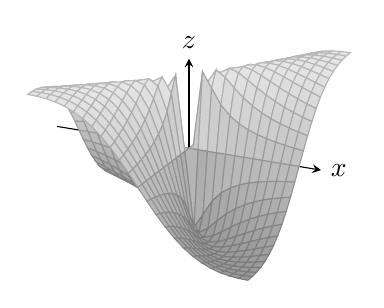
\begin{tikzpicture}[declare function={f(\x,\y)=2*\x*\y/((\x)^2+(\y)^2);}]
  \begin{axis}[small,axis lines=center,colormap={}{gray(0.2cm)=(0.6);gray(1cm)=(0.9);},enlargelimits=true,xlabel={$x$},ylabel={$y$},zlabel={$z$},hide y axis,xlabel style={anchor={west}},zlabel style={anchor=south},xtick={\empty},ytick={\empty},ztick={\empty}]
    \addplot3[surf] { (x==0&&y==0) ?0 : f(x,y) } ;
  \end{axis}
\end{tikzpicture}
\end{subfigure}\hfill
\begin{subfigure}{0.45\textwidth}
\centering
\begin{tikzpicture}[declare function={f(\x,\y)=2*\x*\y/((\x)^2+(\y)^2);}]
  \begin{axis}[small,axis lines=center,colormap={}{gray(0.2cm)=(0.6);gray(1cm)=(0.9);},enlargelimits=true,xlabel={$x$},ylabel={$y$},zlabel={$z$},xlabel style={anchor={west}},ylabel style={anchor=south west},zlabel style={anchor=south},xtick={\empty},ytick={\empty},ztick={\empty},hide z axis]
\addplot3[contour gnuplot={output point meta=rawz,number=5,labels=false,},samples=41,z filter/.code=\def\pgfmathresult{0},]{f(x,y)};
\addplot3[] coordinates {(0,0,0)}coordinate(ka);
  \end{axis}
\draw[fill=white](ka) circle (2pt);
\end{tikzpicture}
\end{subfigure}
\caption{ماسوائے نقطہ \عددی{(0,0)} تفاعل \عددی{f(x,y)} استمراری ہے۔}
\label{شکل_مثال_کثیرالمتغیر_حد_یکتا_ضروری}
\end{figure}

\ابتدا{مثال}\شناخت{مثال_کثیرالمتغیر_حد_یکتا_ضروری}
دکھائیں کہ ماسوائے مبدا   درج ذیل ہر نقطہ پر استمراری ہے (شکل \حوالہ{شکل_مثال_کثیرالمتغیر_حد_یکتا_ضروری})۔
\begin{align*}
f(x,y)=
\begin{cases}
\frac{2xy}{x^2+y^2},&(x,y)\ne (0,0)\\
0,&(x,y)=(0,0)
\end{cases}
\end{align*}
حل:\quad
ہر نقطہ \عددی{(x,y)\ne (0,0)} پر تفاعل کی قیمت \عددی{x} اور \عددی{y}کے  ناطق تفاعل سے حاصل کی جاتی ہے لہٰذا   \عددی{f}   استمراری ہو گا۔

نقطہ \عددی{(0,0)} پر \عددی{f}  کی قیمت معین ہے، لیکن ہم دعویٰ کرتے ہیں کہ \عددی{(x,y)\to(0,0)} کرتے ہوئے اس کا حد غیر موجود ہے۔اس کی وجہ، جیسا ہم دیکھیں گے،   یہ ہے کہ مبدا تک مختلف راہوں سے پہنچتے ہوئے مختلف  نتائج حاصل ہوتے ہیں۔

درج ذیل کی بنا، سوراخ دار لکیر \عددی{y=mx,\, x\ne 0} پر \عددی{m} کی ہر قیمت کے لئے تفاعل \عددی{f} کی ایک مستقل قیمت  ہو گی۔
\begin{align*}
\left. f(x,y)\right\vert_{y=mx}=\left. \frac{2xy}{x^2+y^2}\right\vert_{y=mx}=\frac{2x(mx)}{x^2+(mx)^2}=\frac{2mx^2}{x^2+m^2x^2}=\frac{2m}{1+m^2}
\end{align*}
یوں  اس لکیر  پر جیسے جیسے   \عددی{(x,y)} مبدا تک پہنچتا ہے،  \عددی{f} کی حد اتنی ہو گی:
\begin{align*}
\lim_{\substack{(x,y)\to(0,0)\\ \text{\RL{خط $y=mx$ پر}}}} f(x,y)=\lim_{(x,y)\to(0,0)}\big[\left.f(x,y)\right\vert_{y=mx}\big]=\frac{2m}{1+m^2}
\end{align*}
ہم دیکھتے ہیں کہ حد کی قیمت \عددی{m} پر منحصر ہے۔یوں ایسی کوئی   یکتا قیمت حاصل نہیں ہوتی  جس کو    مبدا تک \عددی{(x,y)} پہنچنے   پر ہم  \عددی{f}  کی حد کہہ سکیں۔ مبدا پر حد غیر موجود ہے لہٰذا مبدا  پر تفاعل غیر استمراری ہو گا۔
\انتہا{مثال}
%=============

دو  (یا دو سے زیادہ)متغیرات کے تفاعل کے حد کے بارے میں ایک اہم نقطہ مثال \حوالہ{مثال_کثیرالمتغیر_حد_یکتا_ضروری} میں  اجاگر ہوا۔ ایک نقطہ پر حد کی موجودگی کے لئے  ضروری ہے کہ اس نقطہ تک  تمام آمد    راہوں  پر  حد  کی قیمت ایک جیسی ہو۔  یوں جب بھی ہم ایک نقطہ  تک  ایسی راہیں  تلاش  کریں جن  پر حد ایک دوسرے سے  مختلف ہوں  تب  اس نقطہ پر تفاعل کا حد غیر موجود ہو گا۔

\ابتدا{پرکھ}\موٹا{حد کی غیر موجودگی کی  دو راہ  پرکھ}\\
اگر \عددی{(x_0,y_0)} تک نقطہ \عددی{(x,y)} ایسی دو مختلف راہوں سے پہنچے جن پر \عددی{f(x,y)} کے حد ایک دوسرے سے مختلف ہوں تب \عددی{\lim\limits_{(x,y)\to(x_0,y_0)}f(x,y)} غیر موجود ہو گا۔
\انتہا{پرکھ}
%===================

\ابتدا{مثال}\شناخت{مثال_کثیرالمتغیر_مبدا_پر_غیر_استمراری_سطح_ب}
دکھائیں کہ \عددی{(0,0)} تک \عددی{(x,y)} پہنچنے سے درج ذیل تفاعل کا کوئی حد حاصل نہیں ہوتا ہے (شکل \حوالہ{شکل_مثال_کثیرالمتغیر_مبدا_پر_غیر_استمراری_سطح_ب})۔
\begin{align*}
f(x,y)=\frac{2x^2y}{x^4+y^2}
\end{align*}
حل:\quad
منحنی \عددی{y=kx^2,\, x\ne 0} پر اس تفاعل کی قیمت ایک مستقل ہے:
\begin{align*}
\left.f(x,y)\right\vert_{y=kx^2}=\left.\frac{2x^2y}{x^4+y^2}\right\vert_{y=kx^2}=\frac{2x^2(kx^2)}{x^4+(kx^2)^2}=\frac{2kx^4}{x^4+k^2x^4}=\frac{2k}{1+k^2}
\end{align*}  
یوں
\begin{align*}
\lim_{\substack{(x,y)\to (0,0)\\ \text{\RL{$y=kx^2$ پر}}}}f(x,y)=\lim_{(x,y)\to(0,0)}\big[\left.f(x,y)\right\vert_{y=kx^2}\big]=\frac{2k}{1+k^2}
\end{align*}
ہو گا  جو   آمد راہ  پر منحصر ہے۔ اگر \عددی{(x,y)} نقطہ \عددی{(0,0)} تک قطع مکافی \عددی{y=x^2}  راہ پر چلتے ہوئے پہنچے، جہاں \عددی{k=1} ہے،  تب حد \عددی{1} کے برابر حاصل ہوتا ہے۔ اگر \عددی{(x,y)} نقطہ \عددی{(0,0)} تک محور \عددی{x} پر چلتے ہوئے پہنچے، جہاں \عددی{k=0} ہے،  تب حد \عددی{0} کے برابر حاصل ہوتا ہے۔ یوں دو راہ پرکھ کے تحت \عددی{(0,0)} تک \عددی{(x,y)} کے پہنچنے سے \عددی{f} کا کوئی حد حاصل نہیں ہو گا۔  
\انتہا{مثال}
%=================
\begin{figure}
\centering
\begin{subfigure}{0.45\textwidth}
\centering
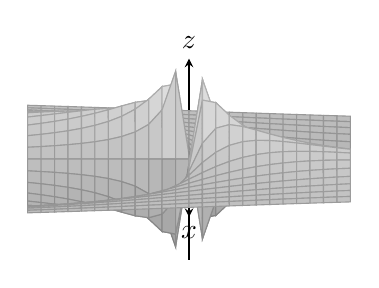
\begin{tikzpicture}[declare function={f(\x,\y)=2*\x*\y/((\x)^4+(\y)^2);}]
  \begin{axis}[view/h=90,small,axis lines=center,colormap={}{gray(0.2cm)=(0.6);gray(1cm)=(0.9);},enlargelimits=true,xlabel={$x$},ylabel={$y$},zlabel={$z$},hide y axis,xlabel style={anchor={north}},zlabel style={anchor=south},xtick={\empty},ytick={\empty},ztick={\empty}]
    \addplot3[surf,domain=-2:2,domain y=-1:1] { (x==0&&y==0) ?0 : f(x,y) } ;
  \end{axis}
\end{tikzpicture}
\end{subfigure}\hfill
\begin{subfigure}{0.45\textwidth}
\centering
\begin{tikzpicture}[declare function={f(\x,\y)=2*\x*\y/((\x)^4+(\y)^2);}]
  \begin{axis}[view/h=90,small,axis lines=center,colormap={kdark}{gray(0.2cm)=(0.6);gray(1cm)=(0.6);},enlargelimits=true,xlabel={$x$},ylabel={$y$},zlabel={$z$},xlabel style={anchor={west}},ylabel style={anchor=south west},zlabel style={anchor=south},xtick={\empty},ytick={\empty},ztick={\empty},hide z axis]
\addplot3[contour gnuplot={output point meta=rawz,number=10,labels=false,},samples=41,z filter/.code=\def\pgfmathresult{0},]{f(x,y)};
  \end{axis}
\end{tikzpicture}
\end{subfigure}
\caption{ماسوائے نقطہ \عددی{(0,0)} تفاعل \عددی{f(x,y)=2x^2y/(x^4+y^2)} استمراری ہے۔}
\label{شکل_مثال_کثیرالمتغیر_مبدا_پر_غیر_استمراری_سطح_ب}
\end{figure}
یہاں آپ سوال اٹھا سکتے ہیں کہ مبدا تک نقطہ \عددی{(x,y)} کے پہنچنے سے بہت سارے مختلف حد ملتے ہیں لہٰذا یہ کہنا درست نہیں کہ \عددی{f} کا حد غیر موجود ہے۔ یہی وہ نقطہ ہے جسے سمجھنا ضروری ہے۔ حد کی تعریف  کہتی ہے کہ حد کی قیمت راہ پر منحصر نہیں ہو سکتی۔

\جزوحصہء{دو سے زیادہ متغیرات کے تفاعل}
دو متغیرات کے تفاعل  کے حد اور استمرار کی تعریف  اور ان  تفاعل کے مجموعہ،  فرق، حاصل ضرب، حاصل تقسیم، طاقت اور مرکب کے بارے میں حاصل نتائج  تین یا تین سے زیادہ متغیرات کے تفاعل کے لئے بھی کارآمد  ہیں۔ درج ذیل تفاعل اپنے پورے دائرہ کار میں استمراری ہیں
\begin{align*}
\ln(x+y+z)\quad \text{اور}\quad \frac{y\sin z}{x-1}
\end{align*} 
اور  درج ذیل طرز کا حد ، جہاں \عددی{N} نقطہ \عددی{(x,y,z)} کو ظاہر کرتا ہے،   حاصل کرنے کے لئے  تفاعل میں نقطہ پر  کیا جاتا ہے۔
\begin{align*}
\lim_{N\to(1,0,-1)}\frac{e^{x+z}}{z^2+\cos\sqrt{xy}}=\frac{e^{1-1}}{(-1)^2+\cos 0}=\frac{1}{2}
\end{align*}

\جزوحصہء{سوالات}
\ابتدا{سوالات}
\موٹا{حد کی قیمت کی تلاش}\\
سوال \حوالہ{سوال_کثیرالمتغیر_حد_قیمت_تلاش_الف} تا سوال \حوالہ{سوال_کثیرالمتغیر_حد_قیمت_تلاش_ب} میں حد کی قیمت تلاش کریں۔

\ابتدا{سوال}\شناخت{سوال_کثیرالمتغیر_حد_قیمت_تلاش_الف}
$\lim\limits_{(x,y)\to(0,0)}\frac{3x^2-y^2+5}{x^2+y^2+2}$
\ابتدا{جواب}
\wf{\unexpanded{
$\tfrac{5}{2}$
}}
\انتہا{جواب}
\انتہا{سوال}
%==================
\ابتدا{سوال}
$\lim\limits_{(x,y)\to(0,4)}\frac{x}{\sqrt{y}}$
\انتہا{سوال}
%===================
\ابتدا{سوال}
$\lim\limits_{(x,y)\to(3,4)}\sqrt{x^2+y^2-1}$
\ابتدا{جواب}
\wf{\unexpanded{
$2\sqrt{6}$
}}
\انتہا{جواب}
\انتہا{سوال}
%===================
\ابتدا{سوال}
$\lim\limits_{(x,y)\to(2,-3)}\big(\frac{1}{x}+\frac{1}{y}\big)^2$
\انتہا{سوال}
%===================
\ابتدا{سوال}
$\lim\limits_{(x,y)\to(0,\pi/4)}\sec x\tan y$
\ابتدا{جواب}
\wf{\unexpanded{
$1$
}}
\انتہا{جواب}
\انتہا{سوال}
%===================
\ابتدا{سوال}
$\lim\limits_{(x,y)\to(0,0)}\cos\frac{x^2+y^3}{x+y+1}$
\انتہا{سوال}
%===================
\ابتدا{سوال}
$\lim\limits_{(x,y)\to(0,\ln 2)}e^{x-y}$
\ابتدا{جواب}
\wf{\unexpanded{
$\tfrac{1}{2}$
}}
\انتہا{جواب}
\انتہا{سوال}
%===================
\ابتدا{سوال}
$\lim\limits_{(x,y)\to(1,1)}\ln\abs{1+x^2y^2}$
\انتہا{سوال}
%===================
\ابتدا{سوال}
$\lim\limits_{(x,y)\to(0,0)} \frac{e^y\sin x}{x}$
\ابتدا{جواب}
\wf{\unexpanded{
$1$
}}
\انتہا{جواب}
\انتہا{سوال}
%===================
\ابتدا{سوال}
$\lim\limits_{(x,y)\to(1,1)}\cos\sqrt[3]{\abs{xy}-1}$
\انتہا{سوال}
%===================
\ابتدا{سوال}
$\lim\limits_{(x,y)\to(1,0)}\frac{x\sin y}{x^2+1}$
\ابتدا{جواب}
\wf{\unexpanded{
$0$
}}
\انتہا{جواب}
\انتہا{سوال}
%===================
\ابتدا{سوال}\شناخت{سوال_کثیرالمتغیر_حد_قیمت_تلاش_ب}
$\lim\limits_{(x,y)\to(\pi/2,0)}\frac{\cos y+1}{y-\sin x}$
\انتہا{سوال}
%===================

\موٹا{حاصل تقسیم کے حد}\\
حاصل تقسیم کو ترتیب دیتے ہوئے سوال \حوالہ{سوال_کثیرالمتغیر_ترتیب_حد_تلاش_الف} تا سوال \حوالہ{سوال_کثیرالمتغیر_ترتیب_حد_تلاش_ب} میں حد تلاش کریں۔

\ابتدا{سوال}\شناخت{سوال_کثیرالمتغیر_ترتیب_حد_تلاش_الف}
$\lim\limits_{\substack{(x,y)\to(1,1)\\ x\ne y}}\frac{x^2-2xy+y^2}{x-y}$
\ابتدا{جواب}
\wf{\unexpanded{
$0$
}}
\انتہا{جواب}
\انتہا{سوال}
%=================
\ابتدا{سوال}
$\lim\limits_{\substack{(x,y)\to(1,1)\\ x\ne y}}\frac{x^2-y^2}{x-y}$
\انتہا{سوال}
%=================
\ابتدا{سوال}
$\lim\limits_{\substack{(x,y)\to(1,1)\\x\ne 1}}\frac{xy-y-2x+2}{x-1}$
\ابتدا{جواب}
\wf{\unexpanded{
$-1$
}}
\انتہا{جواب}
\انتہا{سوال}
%=================
\ابتدا{سوال}
$\lim\limits_{\substack{(x,y)\to(2,-4)\\y\ne -4,\, x\ne x^2}}\frac{y+4}{x^2y-xy+4x^2-4x}$
\انتہا{سوال}
%=================
\ابتدا{سوال}
$\lim\limits_{\substack{(x,y)\to(0,0)\\x\ne y}}\frac{x-y+2\sqrt{x}-2\sqrt{y}}{\sqrt{x}-\sqrt{y}}$
\ابتدا{جواب}
\wf{\unexpanded{
$2$
}}
\انتہا{جواب}
\انتہا{سوال}
%=================
\ابتدا{سوال}
$\lim\limits_{\substack{(x,y)\to(2,2)\\x+y\ne 4}}\frac{x+y-4}{\sqrt{x+y}-2}$
\انتہا{سوال}
%=================
\ابتدا{سوال}
$\lim\limits_{\substack{(x,y)\to(2,0)\\2x-y\ne 4}}\frac{\sqrt{2x-y}-2}{2x-y-4}$
\ابتدا{جواب}
\wf{\unexpanded{
$\tfrac{1}{4}$
}}
\انتہا{جواب}
\انتہا{سوال}
%=================
\ابتدا{سوال}\شناخت{سوال_کثیرالمتغیر_ترتیب_حد_تلاش_ب}
$\lim\limits_{\substack{(x,y)\to(4,3)\\x\ne y+1}}\frac{\sqrt{x}-\sqrt{y+1}}{x-y-1}$
\انتہا{سوال}
%=================

\موٹا{تین متغیرات کے تفاعل کا حد}\\
سوال \حوالہ{سوال_کثیرالمتغیر_تین_متغیر_حد_الف} تا سوال \حوالہ{سوال_کثیرالمتغیر_تین_متغیر_حد_ب} میں حد تلاش کریں۔

\ابتدا{سوال}\شناخت{سوال_کثیرالمتغیر_تین_متغیر_حد_الف}
$\lim\limits_{N\to (1,3,4)}\big(\frac{1}{x}+\frac{1}{y}+\frac{1}{z}\big)$
\ابتدا{جواب}
\wf{\unexpanded{
$\tfrac{19}{12}$
}}
\انتہا{جواب}
\انتہا{سوال}
%=====================
\ابتدا{سوال}
$\lim\limits_{N\to(1,-1,-1)}\frac{2xy+yz}{x^2+z^2}$
\انتہا{سوال}
%================
\ابتدا{سوال}
$\lim\limits_{N\to(3,3,0)}(\sin^2x+\cos^2y+\sec^2z)$
\ابتدا{جواب}
\wf{\unexpanded{
$2$
}}
\انتہا{جواب}
\انتہا{سوال}
%======================
\ابتدا{سوال}
$\lim\limits_{N\to(-1/4,\pi/2,2)}\tan^{-1}xyz$
\انتہا{سوال}
%======================
\ابتدا{سوال}
$\lim\limits_{N\to(\pi,0,3)}ze^{-2y}\cos 2x$
\ابتدا{جواب}
\wf{\unexpanded{
$3$
}}
\انتہا{جواب}
\انتہا{سوال}
%======================
\ابتدا{سوال}\شناخت{سوال_کثیرالمتغیر_تین_متغیر_حد_ب}
$\lim\limits_{N\to(0,-2,0)}\ln\sqrt{x^2+y^2+z^2}$
\انتہا{سوال}
%======================

\موٹا{مستوی میں استمرار}\\
سوال \حوالہ{سوال_کثیرالمتغیر_استمراری_سطح_الف} تا سوال \حوالہ{سوال_کثیرالمتغیر_استمراری_سطح_ب} میں  کس نقطہ \عددی{(x,y)} پر مستوی میں تفاعل استمراری ہیں؟

\ابتدا{سوال}\شناخت{سوال_کثیرالمتغیر_استمراری_سطح_الف}
(ا)
$f(x,y)=\sin(x+y)$\quad
(ب)
$f(x,y)=\ln(x^2+y^2)$
\ابتدا{جواب}
\wf{\unexpanded{
(ا)   تمام \عددی{(x,y)}، (ب) ماسوائے \عددی{(0,0)} تمام \عددی{(x,y)}
}}
\انتہا{جواب}
\انتہا{سوال}
%==================
\ابتدا{سوال}
(ا)
$f(x,y)=\frac{x+y}{x-y}$\quad
(ب)
$f(x,y)=\frac{y}{x^2+1}$
\انتہا{سوال}
%=================
\ابتدا{سوال}
(ا)
$g(x,y)=\sin\frac{1}{xy}$\quad
(ب)
$g(x,y)=\frac{x+y}{2+\cos x}$
\ابتدا{جواب}
\wf{\unexpanded{
(ا) تمام \عددی{(x,y)} ماسوائے جہاں \عددی{x=0} یا \عددی{y=0} ہو، (ب) تمام \عددی{(x,y)}
}}
\انتہا{جواب}
\انتہا{سوال}
%=================
\ابتدا{سوال}\شناخت{سوال_کثیرالمتغیر_استمراری_سطح_ب}
(ا)
$g(x,y)=\frac{x^2+y^2}{x^2-3x+2}$\quad
(ب)
$g(x,y)=\frac{1}{x^2-y}$
\انتہا{سوال}
%=================

\موٹا{فضا میں استمرار}\\
سوال \حوالہ{سوال_کثیرالمتغیر_استمراری_فضا_الف} تا سوال \حوالہ{سوال_کثیرالمتغیر_استمراری_فضا_ب} میں  کس نقطہ \عددی{(x,y,z)} پر فضا  میں تفاعل استمراری ہیں؟

\ابتدا{سوال}\شناخت{سوال_کثیرالمتغیر_استمراری_فضا_الف}
(ا)
$f(x,y,z)=x^2+y^2-2z^2$\quad
(ب)
$f(x,y,z)=\sqrt{x^2+y^2-1}$
\ابتدا{جواب}
\wf{\unexpanded{
(ا) تمام \عددی{(x,y,z)}، (ب) نلکی \عددی{x^2+y^2=1} کی اندرون کے علاوہ تمام \عددی{(x,y,z)}
}}
\انتہا{جواب}
\انتہا{سوال}
%=================
\ابتدا{سوال}
(ا)
$f(x,y,z)=\ln xyz$\quad
(ب)
$f(x,y,z)=e^{x+y}\cos z$
\انتہا{سوال}
%=====================
\ابتدا{سوال}
(ا)
$h(x,y,z)=xy\sin\frac{1}{z}$\quad
(ب)
$h(x,y,z)=\frac{1}{x^2+z^2-1}$
\ابتدا{جواب}
\wf{\unexpanded{
(ا) وہ تمام \عددی{(x,y,z)} جہاں \عددی{z\ne 0} ہو، (ب)   وہ تمام \عددی{(x,y,z)} جہاں \عددی{x^2+y^2\ne 1} ہو۔
}}
\انتہا{جواب}
\انتہا{سوال}
%=====================
\ابتدا{سوال}\شناخت{سوال_کثیرالمتغیر_استمراری_فضا_ب}
(ا)
$h(x,y,z)=\frac{1}{\abs{y}+\abs{z}}$\quad
(ب)
$h(x,y,z)=\frac{1}{\abs{xy}+\abs{z}}$
\انتہا{سوال}
%=====================

\موٹا{نقطہ پر حد غیر موجود}\\
نقطہ تک   مختلف راہ پر پہنچتے ہوئے سوال \حوالہ{سوال_کثیرالمتغیر_غیر_موجود_حد_الف} تا سوال \حوالہ{سوال_کثیرالمتغیر_غیر_موجود_حد_ب} میں دکھائیں کہ \عددی{(x,y)\to(0,0)} کرتے ہوئے تفاعل کا کوئی حد نہیں پایا جاتا ہے۔

\ابتدا{سوال}\شناخت{سوال_کثیرالمتغیر_غیر_موجود_حد_الف}
$f(x,y)=-\frac{x}{\sqrt{x^2+y^2}}$
\begin{center}
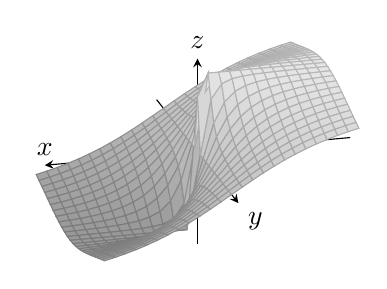
\begin{tikzpicture}[declare function={f(\x,\y)=-\x/sqrt((\x)^2+(\y)^2);}]
\begin{axis}[small,axis lines=center,view/h=165,colormap={}{gray(0.2cm)=(0.6);gray(1cm)=(0.9);},enlargelimits=true,xlabel={$x$},ylabel={$y$},zlabel={$z$},xlabel style={anchor=south},ylabel style={anchor=north west},zlabel style={anchor=south},xtick={\empty},ytick={\empty},ztick={\empty}]
\addplot3[z buffer=sort,surf,domain=-0.1:0.1,domain y=-0.1:0.1]{f(x,y)};
\end{axis}
\end{tikzpicture}
\end{center}
\ابتدا{جواب}
\wf{\unexpanded{
راہ \عددی{y=x,x>0} اور \عددی{y=x,x<0}  لیں۔ 
}}
\انتہا{جواب}
\انتہا{سوال}
%===================
\ابتدا{سوال}
$h(x,y)=\frac{x^4}{x^4+y^2}$
\begin{center}
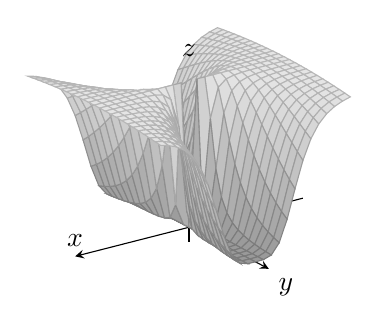
\begin{tikzpicture}[declare function={f(\x,\y)=(\x)^4/((\x)^4+(\y)^2);}]
\begin{axis}[small,axis lines=center,view/h=145,colormap={}{gray(0.2cm)=(0.6);gray(1cm)=(0.9);},enlargelimits=true,xlabel={$x$},ylabel={$y$},zlabel={$z$},xlabel style={anchor=south},ylabel style={anchor=north west},zlabel style={anchor=south},xtick={\empty},ytick={\empty},ztick={\empty}]
\addplot3[z buffer=sort,surf]{f(x,y)};
\end{axis}
\end{tikzpicture}
\end{center}
\انتہا{سوال}
%=================
\ابتدا{سوال}
$h(x,y)=\frac{x^4-y^2}{x^4+y^2}$
\ابتدا{جواب}
\wf{\unexpanded{
راہ \عددی{y=kx^2} لیں جہاں \عددی{k} ایک  مستقل ہو۔
}}
\انتہا{جواب}
\انتہا{سوال}
%================
\ابتدا{سوال}
$f(x,y)=\frac{xy}{\abs{xy}}$
\انتہا{سوال}
%=================
\ابتدا{سوال}
$g(x,y)=\frac{x-y}{x+y}$
\ابتدا{جواب}
\wf{\unexpanded{
راہ \عددی{y=mx} لیں جہاں \عددی{m} ایک مستقل    \عددی{m\ne -1} ہو۔
}}
\انتہا{جواب}
\انتہا{سوال}
%=================
\ابتدا{سوال}
$g(x,y)=\frac{x+y}{x-y}$
\انتہا{سوال}
%=================
\ابتدا{سوال}
$h(x,y)=\frac{x^2+y}{y}$
\ابتدا{جواب}
\wf{\unexpanded{
راہ \عددی{y=kx^2} لیں جہاں \عددی{k} ایک مستقل  \عددی{k\ne 0} ہو۔ 
}}
\انتہا{جواب}
\انتہا{سوال}
%=================
\ابتدا{سوال}\شناخت{سوال_کثیرالمتغیر_غیر_موجود_حد_ب}
$h(x,y)=\frac{x^2}{x^2-y}$
\انتہا{سوال}
%=================
\موٹا{نظریہ اور مثالیں}\\
\ابتدا{سوال}
کیا  \عددی{\lim_{(x,y)\to(x_0,y_0)}f(x,y)=L} کی صورت میں \عددی{(x_0,y_0)} کا معین ہونا لازمی ہے؟ اپنے جواب کی وجہ پیش کریں۔
\ابتدا{جواب}
\wf{\unexpanded{
نہیں
}}
\انتہا{جواب}
\انتہا{سوال}
%=====================
\ابتدا{سوال}
اگر \عددی{f(x_0,y_0)=3} ہو تب درج ذیل کے بارے میں  (ا)   \عددی{(x_0,y_0)} پر استمراری \عددی{f} کی صورت میں،
\begin{align*}
\lim_{(x,y)\to(x_0,y_0)} f(x,y)
\end{align*}
(ب)  \عددی{(x_0,y_0)} پر غیر استمراری \عددی{f} کی صورت میں کیا کہا جا  سکتا ہے۔ اپنے جواب کہ وجہ پیش کریں۔
\انتہا{سوال}
%===============
دو متغیرات کے تفاعل کا مسئلہ بیچ  کہتا ہے کہ اگر ایک قرص، جس کا  مرکز  \عددی{(x_0,y_0)} ہو، کے اندر تمام \عددی{(x,y)\ne (x_0,y_0)} پر \عددی{g(x,y)\le f(x,y)\le h(x,y)} ہو،  اور \عددی{(x,y)\to (x_0,y_0)} کرتے ہوئے  \عددی{g} اور \عددی{h} دونوں کا  حد  متناہی اور \عددی{L} ہو   تب
\begin{align*}
\lim_{(x,y)\to(x_0,y_0)}f(x,y)=L
\end{align*}
ہو گا۔سوال \حوالہ{سوال_کثیرالمتغیر_مسئلہ_بیچ_الف} تا سوال \حوالہ{سوال_کثیرالمتغیر_مسئلہ_بیچ_ب} میں  اس نتیجہ  کا سہارا لیتے ہوئے جواب دیں۔ 

\ابتدا{سوال}\شناخت{سوال_کثیرالمتغیر_مسئلہ_بیچ_الف}
کیا 
\begin{align*}
1-\frac{x^2y^2}{3}<\frac{\tan^{-1}xy}{xy}<1
\end{align*}
جانتے ہوئے آپ
\begin{align*}
\lim\limits_{(x,y)\to(0,0)}\frac{\tan^{-1}xy}{xy}
\end{align*}
کے بارے میں کچھ کہہ سکتے ہیں؟ اپنے جواب کی وجہ پیش کریں۔
\ابتدا{جواب}
\wf{\unexpanded{
حد \عددی{1} ہے۔
}}
\انتہا{جواب}
\انتہا{سوال}
%============
\ابتدا{سوال}
کیا
\begin{align*}
2\abs{xy}-\frac{x^2y^2}{6}<4-4\cos\sqrt{\abs{xy}}<2\abs{xy}
\end{align*}
جانتے ہوئے
\begin{align*}
\lim\limits_{(x,y)\to(0,0)}\frac{4-4\cos\sqrt{\abs{xy}}}{\abs{xy}}
\end{align*}
کے بارے میں کچھ کہا جا سکتا ہے؟ اپنے جواب کی وجہ پیش کریں۔
\انتہا{سوال}
%===============
\ابتدا{سوال}
کیا \عددی{\abs{\sin(1/x)}\le 1} جانتے ہوئے درج ذیل کے بارے میں کچھ کہا جا سکتا ہے؟ اپنے جواب کی وجہ پیش کریں۔
\begin{align*}
\lim\limits_{(x,y)\to(0,0)}y\sin\frac{1}{x}
\end{align*}
\ابتدا{جواب}
\wf{\unexpanded{
حد \عددی{0} ہے۔
}}
\انتہا{جواب}
\انتہا{سوال}
%==============
\ابتدا{سوال}
کیا \عددی{\abs{\cos(1/y)}\le 1} جانتے ہوئے درج ذیل کے بارے میں کچھ کہا جا سکتا ہے؟ اپنے جواب کی وجہ پیش کریں۔
\begin{align*}
\lim\limits_{(x,y)\to(0,0)}x\cos\frac{1}{y}
\end{align*}
\انتہا{سوال}
%==============
\ابتدا{سوال}
(ا)دوبارہ  مثال \حوالہ{مثال_کثیرالمتغیر_حد_یکتا_ضروری} کو  پڑھیں۔اب درج ذیل کلیہ میں \عددی{m=\tan\theta} پر کر کے اس کی سادہ صورت حاصل کرتے ہوئے دکھائیں کہ \عددی{f} کی قیمت  لکیر کے زاویہ میلان  پر منحصر ہی گی۔
\begin{align*}
\left.f(x,y)\right\vert_{y=mx}=\frac{2m}{1+m^2}
\end{align*}
(ب) جزو-ا میں حاصل کلیہ استعمال کرتے ہوئے دکھائیں کہ لکیر \عددی{y=mx} پر چلتے ہوئے \عددی{(x,y)\to (0,0)} کرنے سے \عددی{f} کے  حد کی قیمت \عددی{-1} تا \عددی{1} ہو سکتی ہے جو قریب پہنچنے کی راہ کے  زاویہ پر منحصر ہو گی۔  
\ابتدا{جواب}
\wf{\unexpanded{
(ا) \عددی{\left. f(x,y)\right\vert_{y=mx}=\sin2\theta} جہاں\\  
 \عددی{\tan\theta=m} ہے۔
}}
\انتہا{جواب}
\انتہا{سوال}
%=================
\ابتدا{سوال}\شناخت{سوال_کثیرالمتغیر_مسئلہ_بیچ_ب}
\عددی{f(0,0)} کی ایسی تعریف پیش کریں جو درج ذیل کو مبدا پر بھی استمراری بناتا ہو۔
\begin{align*}
f(x,y)=xy\frac{x^2-y^2}{x^2+y^2}
\end{align*}
\انتہا{سوال}
%==============

\موٹا{قطبی محدد میں تبادلہ}\\
اگر کارتیسی محدد میں \عددی{\lim_{(x,y)\to(0,0)}f(x,y)}  کے حصول میں پیش رفت  نہ ہو تب قطبی محدد میں حد تلاش کرنے کی کوشش کریں۔ ایسا کرنے  کی خاطر \عددی{x=r\cos\theta} اور \عددی{y=r\sin\theta} کرتے ہوئے \عددی{r\to 0}  کے لئے حاصل تفاعل کا حد تلاش کریں۔دوسرے الفاظ میں یہ دیکھنے کی کوشش کریں کہ آیا کوئی ایسا عدد \عددی{L} پایا جاتا ہے جو درج ذیل کو مطمئن کرتا ہو:

کسی بھی دیے گئے عدد \عددی{\epsilon>0} کا ایسا مطابقتی عدد \عددی{\delta>0} پایا جاتا ہو کہ تمام \عددی{r} اور \عددی{\theta} کے لئے درج ذیل ہو۔
\begin{align*}
\abs{r}<\delta\implies \abs{f(r,\theta)-L}<\epsilon
\end{align*}
اگر ایسا \عددی{L} موجود ہو تب
\begin{align}\label{مساوات_کثیرالمتغیر_قطبی_حد_الف}
\lim_{(x,y)\to(0,0)}f(x,y)=\lim_{r\to 0}f(r,\theta)=L
\end{align}
ہو گا۔مثال کے طور پر 
\begin{align*}
\lim_{(x,y)\to(0,0)}\frac{x^3}{x^2+y^2}=\lim_{r\to 0}\frac{r^3\cos^3\theta}{r^2}=\lim_{r\to 0}r\cos^3\theta=0
\end{align*}
ہو گا۔ آخری عدم مساوات  کی تصدیق کرنے کی خاطر ہمیں دکھانا  ہو گا کہ \عددی{f(r,\theta)=r\cos^3\theta} اور \عددی{L}  مساوات \حوالہ{مساوات_کثیرالمتغیر_قطبی_حد_الف} کو مطمئن کرتے ہیں۔ یعنی ہمیں دکھانا ہو گا کہ کسی بھی دیے گئے عدد \عددی{\epsilon>0} کے لئے ایسا مطابقتی  عدد \عددی{\delta>0} موجود ہے کہ  تمام \عددی{r} اور \عددی{\theta} کے لئے درج ذیل  مطمئن ہو۔
\begin{align}\label{مساوات_کثیرالمتغیر_قطبی_حد_ب}
\abs{r}<\delta\implies \abs{r\cos^3\theta-0}<\epsilon
\end{align}
چونکہ
\begin{align*}
\abs{r\cos^3\theta}=\abs{r}\abs{\cos^3\theta}\le \abs{r}\cdot 1=\abs{r}
\end{align*}
ہوتا ہے لہٰذا  \عددی{\delta=\epsilon} لینے سے تمام \عددی{r} اور \عددی{\theta} کے لئے مساوات \حوالہ{مساوات_کثیرالمتغیر_قطبی_حد_ب} مطمئن ہو گا۔

اس کے برعکس    \عددی{\abs{r}} جتنا بھی چھوٹا کیوں نا ہو   درج ذیل تفاعل کی قیمت \عددی{0}  سے  \عددی{1} تک ہو سکتی ہے لہٰذا \عددی{\lim_{(x,y)\to (0,0)}\tfrac{x^2}{x^2+y^2}} غیر موجود ہو گا۔
\begin{align*}
\frac{x^2}{x^2+y^2}=\frac{r^2\cos^2\theta}{r^2}=\cos^2\theta
\end{align*}

درج بالا دو تفاعل میں \عددی{r\to 0} کرتے ہوئے  حد کی موجودگی یا غیر موجودگی کا مسئلہ سیدھا تھا۔البتہ ضروری نہیں کہ  قطبی محدد میں تبادلہ سودمند ثابت ہو، بلکہ بعض اوقات ایسا کرنے سے ہم بالکل غلط نتیجہ کی طرف راغب ہو سکتے ہیں۔ مثال کے طور پر، تمام سیدھے خطوط \عددی{\theta=c}، جہاں \عددی{c} مستقل ہے، پر حد موجود ہو سکتا ہے اگرچہ وسیع معنوں میں حد غیر موجود ہو گا۔ مثال \حوالہ{مثال_کثیرالمتغیر_مبدا_پر_غیر_استمراری_سطح_ب} میں اس حقیقت کی وضاحت کی گئی ہے۔قطبی محدد میں \عددی{r\ne 0} کے لئے  \عددی{f(x,y)=\tfrac{2x^2y}{x^4+y^2}} درج ذیل ہو گا۔
\begin{align*}
f(r\cos\theta,r\sin\theta)=\frac{r\cos\theta\sin2\theta}{r^2\cos^4\theta+\sin^2\theta}
\end{align*}
اب \عددی{\theta}  برقرار رکھتے ہوئے  \عددی{r\to 0} کرنے سے حد \عددی{0} ملتا ہے۔البتہ راہ \عددی{y=x^2} پر \عددی{r\sin\theta=r^2\cos^2\theta}لہٰذا درج ذیل ہو گا۔
\begin{align*}
f(r\cos\theta,r\sin\theta)&=\frac{r\cos\theta\sin 2\theta}{r^2\cos^4\theta+(r\cos^2\theta)^2}\\
&=\frac{2r\cos^2\theta\sin\theta}{2r^2\cos^4\theta}=\frac{r\sin\theta}{r^2\cos^2\theta}=1
\end{align*}

سوال \حوالہ{سوال_کثیرالمتغیر_قطبی_محدد_حد_الف} تا سوال \حوالہ{سوال_کثیرالمتغیر_قطبی_محدد_حد_ب} میں \عددی{(x,y)\to(0,0)} کرتے ہوئے \عددی{f} کا حد تلاش کریں یا دکھائیں کہ اس کا حد غیر موجود ہے۔

\ابتدا{سوال}\شناخت{سوال_کثیرالمتغیر_قطبی_محدد_حد_الف}
$f(x,y)=\frac{x^3-xy^2}{x^2+y^2}$
\ابتدا{جواب}
\wf{\unexpanded{
$0$
}}
\انتہا{جواب}
\انتہا{سوال}
%==================
\ابتدا{سوال}
$f(x,y)=\cos\big(\frac{x^3-y^3}{x^2+y^2}\big)$
\انتہا{سوال}
%====================
\ابتدا{سوال}
$f(x,y)=\frac{y^2}{x^2+y^2}$
\ابتدا{جواب}
\wf{\unexpanded{
غیر موجود ہے۔
}}
\انتہا{جواب}
\انتہا{سوال}
%====================
\ابتدا{سوال}
$f(x,y)=\frac{2x}{x^2+x+y^2}$
\انتہا{سوال}
%====================
\ابتدا{سوال}
$f(x,y)=\tan^{-1}\big(\frac{\abs{x}+\abs{y}}{x^2+y^2}\big)$
\ابتدا{جواب}
\wf{\unexpanded{
$\tfrac{\pi}{2}$
}}
\انتہا{جواب}
\انتہا{سوال}
%====================
\ابتدا{سوال}\شناخت{سوال_کثیرالمتغیر_قطبی_محدد_حد_ب}
$f(x,y)=\frac{x^2-y^2}{x^2+y^2}$
\انتہا{سوال}
%====================

سوال \حوالہ{سوال_کثیرالمتغیر_مبدا_پر_استمراری_الف} اور سوال \حوالہ{سوال_کثیرالمتغیر_مبدا_پر_استمراری_ب} میں \عددی{f(0,0)} کی ایسی تعریف پیش کریں کہ \عددی{f} مبدا پر بھی استمراری ہو۔

\ابتدا{سوال}\شناخت{سوال_کثیرالمتغیر_مبدا_پر_استمراری_الف}
$f(x,y)=\ln\big(\frac{3x^2-x^2y^2+3y^2}{x^2+y^2}\big)$
\ابتدا{جواب}
\wf{\unexpanded{
$f(0,0)=\ln 3$
}}
\انتہا{جواب}
\انتہا{سوال}
%====================
\ابتدا{سوال}\شناخت{سوال_کثیرالمتغیر_مبدا_پر_استمراری_ب}
$f(x,y)=\frac{2xy^2}{x^2+y^2}$
\انتہا{سوال}
%=================

\موٹا{\عددی{\delta\epsilon}  تعریفات  کا استعمال}\\
\ابتدا{سوال}
دکھائیں کہ حد کی تعریف  (مساوات \حوالہ{مساوات_کثیرالمتغیر_تعریف_حد_الف}) میں \عددی{\delta\epsilon} پر عائد  شرط مساوات \حوالہ{مساوات_کثیرالمتغیر_تعریف_حد_ب} میں دی گئی شرط کے مترادف ہے۔
\انتہا{سوال}
%===================
\ابتدا{سوال}
\عددی{(x,y)\to (x_0,y_0)} کرتے ہوئے تفاعل \عددی{f(x,y)}کے حد  کی باضابطہ \عددی{\delta\epsilon} تعریف کو مد نظر رکھتے ہوئے  \عددی{(x,y,z)\to(x_ 0,y_0,z_0)} کرتے ہوئے \عددی{g(x,y,z)} کے حد کی تعریف پیش کریں۔چار غیر تابع متغیرات کے تفاعل \عددی{h(x,y,z,t)} کی حد کی تعریف کیا ہو گی؟  
\انتہا{سوال}
%=========

سوال \حوالہ{سوال_کثیرالمتغیر_حد_دو_متغیرات_الف} تا سوال \حوالہ{سوال_کثیرالمتغیر_حد_دو_متغیرات_ب} میں  تفاعل \عددی{f(x,y)} اور مثبت عدد \عددی{\epsilon} دیے گئے ہیں۔ ہر ایک سوال میں یا دکھائیں کہ  ایسا \عددی{\delta>0} موجود ہے  کہ  \عددی{(x,y)} کے لئے 
\begin{align*}
\sqrt{x^2+y^2}<\delta\implies \abs{f(x,y)-f(0,0)}<\epsilon
\end{align*}
مطمئن ہوتا ہے  یا دکھائیں کہ ایسا \عددی{\delta>0} موجود ہے کہ تمام \عددی{(x,y)} کے لئے
\begin{align*}
\abs{x}<\delta,\quad \abs{y}<\delta \implies \abs{f(x,y)-f(0,0)}<\epsilon
\end{align*}
مطمئن ہوتا ہے۔ان میں سے وہ دکھائیں  جو آپ کو زیادہ  آسان لگے۔ دونوں دکھانے  کی ضرورت نہیں ہے۔ 

\ابتدا{سوال}\شناخت{سوال_کثیرالمتغیر_حد_دو_متغیرات_الف}
$f(x,y)=x^2+y^2,\quad \epsilon=0.01$
\ابتدا{جواب}
\wf{\unexpanded{
$\delta=0.1$
}}
\انتہا{جواب}
\انتہا{سوال}
%==================
\ابتدا{سوال}
$f(x,y)=\frac{y}{x^2+1},\quad \epsilon=0.05$
\انتہا{سوال}
%==============
\ابتدا{سوال}
$f(x,y)=\frac{x+y}{x^2+1},\quad \epsilon=0.01$
\ابتدا{جواب}
\wf{\unexpanded{
$\delta=0.005$
}}
\انتہا{جواب}
\انتہا{سوال}
%================
\ابتدا{سوال}\شناخت{سوال_کثیرالمتغیر_حد_دو_متغیرات_ب}
$f(x,y)=\frac{x+y}{2+\cos x},\quad \epsilon=0.02$
\انتہا{سوال}
%=================


سوال \حوالہ{سوال_کثیرالمتغیر_حد_تین_متغیرات_الف} تا سوال \حوالہ{سوال_کثیرالمتغیر_حد_تین_متغیرات_ب} میں  تفاعل \عددی{f(x,y,z)} اور مثبت عدد \عددی{\epsilon} دیے گئے ہیں۔ ہر ایک سوال میں یا دکھائیں کہ  ایسا \عددی{\delta>0} موجود ہے  کہ  \عددی{(x,y,z)} کے لئے 
\begin{align*}
\sqrt{x^2+y^2+z^2}<\delta\implies \abs{f(x,y,z)-f(0,0,0)}<\epsilon
\end{align*}
مطمئن ہوتا ہے  یا دکھائیں کہ ایسا \عددی{\delta>0} موجود ہے کہ تمام \عددی{(x,y,z)} کے لئے
\begin{align*}
\abs{x}<\delta,\quad \abs{y}<\delta,\quad \abs{z}<\delta  \implies \abs{f(x,y,z)-f(0,0,0)}<\epsilon
\end{align*}
مطمئن ہوتا ہے۔ان میں سے وہ دکھائیں  جو آپ کو زیادہ  آسان لگے۔ دونوں دکھانے کی ضرورت نہیں ہے۔ 

\ابتدا{سوال}\شناخت{سوال_کثیرالمتغیر_حد_تین_متغیرات_الف}
$f(x,y,z)=x^2+y^2+z^2,\quad \epsilon=0.015$
\ابتدا{جواب}
\wf{\unexpanded{
$\delta=\sqrt{0.015}$
}}
\انتہا{جواب}
\انتہا{سوال}
%=================
\ابتدا{سوال}
$f(x,y,z)=xyz,\quad \epsilon=0.008$
\انتہا{سوال}
%===================
\ابتدا{سوال}
$f(x,y,z)=\frac{x+y+z}{x^2+y^2+z^2+1},\quad \epsilon=0.015$
\ابتدا{جواب}
\wf{\unexpanded{
$\delta=0.005$
}}
\انتہا{جواب}
\انتہا{سوال}
%===================
\ابتدا{سوال}\شناخت{سوال_کثیرالمتغیر_حد_تین_متغیرات_ب}
$f(x,y,z)=\tan^2x+\tan^2y+\tan^2z,\quad \epsilon=0.03$
\انتہا{سوال}
%===================
\ابتدا{سوال}
دکھائیں کہ ہر نقطہ  \عددی{(x_0,y_0,z_0)} پر تفاعل \عددی{f(x,y,z)=x+y-z} استمراری ہے۔ 
\انتہا{سوال}
%===============
\ابتدا{سوال}
دکھائیں کہ مبدا پر \عددی{f(x,y,z)=x^2+y^2+z^2} استمراری ہے۔
\انتہا{سوال}
%==================
\انتہا{سوالات}

